\chapter{Konzeption und Aufbau des Prototyps}\label{sec:concept}
Nachdem in der Literaturrecherche (Kapitel \textit{\nameref{sec:related-works}}) zentrale funktionale und gestalterische Anforderungen identifiziert und in Kapitel \textit{\nameref{sec:analysis}} vergleichbare Spiele hinsichtlich ihres Game- und Rätseldesigns analysiert wurden, kann \say{Connecting-Minds} nun auf Basis dieser Erkenntnisse vollständig konzipiert werden. Ergänzend fließen die von \cite{krekhov_puzzles_2021} entwickelte Taxonomie für analoge und digitale Escape-Room-Spiele in den Gestaltungsprozess mit ein.

Die Konzeption des Spiels folgt einem systematisch-methodischen Vorgehen. Zunächst werden die übergeordneten Designvision sowie die grundlegenden Zielsetzungen erläutert. Darauf aufbauend dient das \ac{MDA}-Framework (vgl. \citealp{hunicke_mda_2004}) als zentrales Analyse- und Strukturierungsinstrument, um die angestrebte Spielerfahrung gezielt gestalten zu können. In diesem Rahmen werden die grundlegenden Spielmechaniken, die Rollenverteilung sowie die angestrebten dynamischen Prozesse beschrieben. Im Anschluss folgen die Darstellung der technischen Verbundenheit der Anwendungen, das Konzept für das Tutorial, Überlegungen zum Dialog- und Sounddesign sowie eine abschließende Reflexion über die Ideen und Ansätze, die im finalen Prototyp keine Berücksichtigung mehr gefunden haben.

\section{Designziele und Zielgruppe}
Connecting-Minds verfolgt das Ziel, kooperative Kommunikation unter asymmetrischen Perspektiven in einem Escape-Room-ähnlichen Szenario zu fördern. Das Spiel basiert auf der Zusammenarbeit zweier Rollen, Player und Watcher, die gemeinsam Rätsel lösen und Hindernisse in der Spielwelt überwinden müssen. Beide Rollen verfügen über unterschiedliche Wahrnehmungen und Interaktionsmöglichkeiten innerhalb der Spielwelt, die sich gegenseitig ergänzen und auf Kooperation angewiesen sind.

Das Spiel lässt sich dem Genre der kooperativen Adventure-Spiele zuordnen. Außerdem soll es sich dabei, wie im ersten Konzept des Vorabprojekts, um ein \ac{Sci-Fi} Abenteuer handeln.

Im Zentrum des spielerischen Erlebnisses steht die gezielte Verteilung asymmetrischer Informationen, um eine Balance zwischen Orientierung und Vertrauen zu schaffen. Der gemeinsame Fortschritt bildet dabei den zentralen Motivationsfaktor.

Die Zielgruppe entspricht derjenigen, die bereits in der vorangegangenen Konzeptionsphase im Rahmen des Moduls Interaktionsdesign im \ac{UCD}-Prozess entwickelt wurde. Im Fokus stehen drei exemplarische Personae:

\begin{itemize}
    \item \textbf{Steve Works}, 19 Jahre alt, ist Studienganganfänger im Fach Medieninformatik. Neben seinem akademischen Interesse sucht er gezielt nach sozialer Interaktion. Spieleabende und gemeinschaftliche Aktivitäten betrachtet er als Möglichkeit, Kontakte zu knüpfen und den Studienalltag aktiv zu gestalten.
    \item \textbf{Uwe Kaufmann}, 64 Jahre alt, ist erfahrener Projektleiter. Er steht vor der Aufgabe, ein neues Team zusammenzustellen und sieht in \say{Connecting-Minds} eine Gelegenheit, Teambuilding und Motivation zu fördern, um eine effektive Zusammenarbeit zu etablieren.
    \item \textbf{Anja Gayms}, 31 Jahre alt, arbeitet als introvertierte Zahnarzthelferin. Sie sucht im Spiel sowohl eine kognitive Herausforderung als auch eine Gelegenheit, bestehende Freundschaften zu vertiefen.
\end{itemize}

Die vollständige Ausarbeitung der Personae befinden sich im Anhang \ref{sec:append_concept_personae}: \nameref{sec:append_concept_personae}.

\section{Narratives und funktionales Grundgerüst}
Das Spiel basiert auf einem asymmetrischen Zwei-Rollen-Prinzip, bei dem zwei Spieler unterschiedliche Rollen einnehmen und gemeinsam innerhalb einer geteilten Spielwelt agieren. Diese Welt ist in mehrere räumlich und funktional voneinander abgegrenzte Abschnitte gegliedert. Der Fortschritt im Spiel wird durch kooperatives Handeln und das gemeinsame Lösen von Rätsel ermöglicht. Dabei ist die wechselseitige Abhängigkeit beider Rollen wesentlich für das Vorankommen.

Die narrative Struktur des Spiels entfaltet sich durch eine Kombination aus textbasierten Hinweisen, Umweltinformationen und der räumlichen Gestaltung. Das Storytelling ist dabei stark an das sog. \say{Environmental Storytelling} angelehnt, bei dem die Umgebung selbst narrative Funktionen übernimmt.

Die zugrundeliegende Hintergrundgeschichte lautet wie folgt:

Der Protagonist des Spiels nimmt an einer experimentellen Simulation innerhalb seines Forschungsinstituts teil. Diese Simulation verläuft jedoch nicht wie geplant. Durch eine unerwartete Anomalie während des Prozesses wird das Selbst des Protagonisten gespalten. Zurück bleibt der physische Körper in der realen Welt, während das Bewusstsein in das digitale Netz der Forschungseinrichtung übertragen wird. Beide Entitäten, Körper und Geist, existieren fortan getrennt, können jedoch auf bislang unerklärliche Weise miteinander kommunizieren. Ziel beider Instanzen ist es, die Ursache der Anomalie zu ergründen, den oder die Verantwortlichen ausfindig zu machen und schließlich die eigene Wiedervereinigung herbeizuführen.

Die Spielwelt bildet diesen narrativen Rahmen architektonisch und funktional ab. Beginnend in einem alten, unterirdischen Gewölbe des Forschungsinstituts, in das der leibliche Körper nach dem fehlgeschlagenen Experiment gebracht wurde, arbeiten sich die beiden Rollen durch verschiedene Abteilungen der Einrichtung. Dabei sammeln sie Hinweise auf die Hintergründe des Vorfalls und identifizieren mögliche Antagonisten. Im weiteren Verlauf öffnet sich die Spielwelt sukzessive. Sie führt zunächst durch unterschiedliche Gebäudeteile der Forschungseinrichtung, anschließend in Außenareale sowie in die privaten Wohnräume von Personen, die in den Vorfall verwickelt sein könnten. Die Erweiterung der Spielwelt entsteht dabei stets im direkten Zusammenhang mit dem narrativen Fortschritt.


\section{Spielkonzeption mithilfe des MDA-Frameworks}

Aus den bisherigen Recherchen zu asymmetrischen kooperativen Spielen und der zugrunde liegenden Spielerkommunikation geht hervor, dass zwischen den Spielerrollen eine funktionale oder perspektivische Abhängigkeit bestehen muss. Diese Abhängigkeit sollte jedoch nicht zu stark ausgeprägt sein, da ansonsten der Spielfluss beeinträchtigt und Frustration bei den Spielenden hervorgerufen werden könnte. Eine gelungene Balance zwischen Abhängigkeit und Eigenständigkeit der Rollen ist somit essenziell für ein kooperatives und motivierendes Spielerlebnis.

Die Analyse verwendeter Spielkonzepte verdeutlicht, dass bestimmte Inhalte und Funktionalitäten sinnvoll integriert werden können, Gleichzeitig muss jedoch vermieden werden, dass die Rollen zu stark voneinander entkoppelt agieren, da dies die kooperative Interaktion minimieren würde.

Die Spielreihe We were here zeigt, dass Rätselelemente so gestaltet sein müssen, dass sie durch die jeweils andere Spielpartei beschrieben und nachvollziehbar erklärt werden können. Zusätzlich zeigt sich, dass eine höhere Interaktionsdynamik zwischen den Anwendungen der beiden Rollen dazu beiträgt, eine engere Verzahnung von Spielerfahrung und Spielmechanik zu erreichen.

Das Spiel Tiny Room Stories demonstriert, wie sich kleinere Rätselelemente und das schrittweise Freischalten von Hindernissen zu einem übergeordneten Ziel zusammenfügen lassen. Darüber hinaus dient er als Inspirationsquelle hinsichtlich der Steuerungsmechanik und der intuitiven Benutzerführung.

The Past Within macht deutlich, dass ein zu hohes kognitives Anforderungsniveau einzelner Anwendungen die kooperative Kommunikation negativ beeinflussen kann. In solchen Fällen neigen Spieler dazu, sich ausschließlich auf ihre eigene Anwendung zu konzentrieren, wodurch die Sensibilität für kooperative Momente, als Zeitpunkte, an denen die Unterstützung durch die andere Rolle notwendig wäre, verloren geht.

Myrmidon hingegen zeigt, wie stark voneinander abhängige Anwendungsbereiche grundsätzlich gestaltet werden können. Allerdings leidet in diesem Fall das Spielerlebnis unter einer unausgewogenen Rollenverteilung. Die Spielerrolle des Animators nimmt vorwiegend eine unterstützende Funktion für die andere Rolle (die Stop-Motion-Puppe) ein und hat dadurch nur eingeschränkt eigene Spielanteile.

Ein ähnliches Ungleichgewicht lässt sich bei Keep Talking and Nobody Explodes beobachten. Auch hier übernimmt die Expertenrolle hauptsächlich eine beratende Funktion für den Bombenentschärfer, ohne selbst unmittelbar in das Spielgeschehen eingebunden zu sein.

\subsection{Mechanics}
Die mechanischen Elemente des Spiels lassen sich in drei Kategorien einteilen: Die Spielerrolle des Players, die des Watchers sowie allgemeingültige Weltregeln, die für beide Rollen relevant sind.

\paragraph{Player}

Der Player steuert seinen Avatar in der Spielwelt entweder über eine klassische Maussteuerung im Point-and-Click-Stil oder über Touch-Inputs. Die Kameraperspektive kann über das Mausrad bzw. Zoom-Gesten angepasst werden und zwischen einer standardmäßigen isometrischen Ansicht und einer First-Person-Perspektive wechseln.

Das \ac{UI} des Players umfasst eine Toolbar, über welch Interaktionen mit Weltobjekten ausgelöst werden, etwa das Aufnehmen oder Platzieren von Gegenständen. Zusätzlich ist es dem Player möglich, bestimmte Objekte zu tragen und an den Watcher zu übermitteln. Über die First-Person-Ansicht können Gegenstände präzise in der Spielwelt platziert werden.

Neue Objekte in der Spielwelt werden durch physische Annäherung des Avatars freigeschaltet, sobald eine Interaktion möglich ist.

\paragraph{Watcher}

Der Watcher interagiert über eine \ac{AR}-Anwendung mit der Spielwelt, die im physischen Raum vor ihm verankert ist. Er kann sich frei um die virtuelle Szene bewegen und erhält eine übergeordnete Perspektive auf die Raumstruktur sowie auf platzierte oder gesammelte Objekte.

Die Hauptaufgabe des Watchers besteht in der Verwaltung des Objektinventars, dem Platzieren und Entfernen interaktiver Gegenstände sowie dem gezielten weiterleiten von Objekten an den Player. Entfernte Gegenstände wandern zurück in ein Inventar, auf das ausschließlich der Watcher Zugriff hat. Über Touch-Inputs kann er Objekte an beliebige Stellen in der Spielwelt positionieren.

Im späteren Verlauf erhält der Watcher zudem die Möglichkeit, Gegenstände zu skalieren oder zu rotieren.

\paragraph{Weltregeln}

Leichte Gegenstände können vom Player aufgenommen, getragen und entweder über die Interaktionsleiste oder in der First-Person-Ansicht platziert werden. Schwere Objekte hingegen können ausschließlich vom Watcher positioniert, skaliert und rotiert werden, während der Player mit ihnen lediglich interagieren, sie aber nicht tragen kann. 

Sobald ein Gegenstand entdeckt oder in der Spielwelt platziert wurde, kann er vom Watcher (wieder) entfernt und dem Inventar hinzugefügt werden.

Darüber hinaus existieren Hinweise in Form von Texten oder Bildern, die der Player in der Spielwelt entdecken und zur weiteren Analyse an den Watcher weiterleiten kann. Diese Hinweise ergänzen das räumliche eingebettete Rätseldesign der Umgebung und fördern die kooperative Interaktion zwischen den beiden Rollen.

\subsection{Dynamics}

Die aus den Spielmechaniken resultierenden Dynamiken beruhen auf der asymmetrischen Verteilung von Perspektiven und Informationen zwischen den beiden Spielerrollen. Während des Player primär aus der Spielwelt heraus handelt, nimmt der Watcher eine übergeordnete, räumlich flexible Perspektive ein. Diese Asymmetrie bedingt, dass beide Rollen jeweils unterschiedliche Informationen erhalten und diese eigenständig, aber koordiniert interpretieren müssen.

Die Lösung von Herausforderungen erfordert somit die Kombination und wechselseitige Abstimmung beider Spielerfähigkeiten. Nur durch die koordinierte Nutzung der jeweils verfügbaren Informationen und Interaktionsmöglichkeiten entsteht ein funktionierendes kooperatives Zusammenspiel, dass das Fortschreiten im Spiel ermöglicht.

Besonders hervorzuheben ist die räumliche Dynamik, die durch den Einsatz der \ac{AR}-Technologie entsteht. Die Spielwelt wird in den physischen Raum des Watchers projiziert, wodurch eine neuartige räumliche Orientierung und Interaktionsform entsteht, die über klassische Bildschirmdarstellung hinausgeht. Diese physisch-virtuelle Verschmelzung unterstützt nicht nur die Immersion, sondern verstärkt auch die Notwendigkeit einer engen Abstimmung zwischen den Spielerrollen.

\subsection{Aesthetics}

Das Spiel adressiert die ästhetischen Dimensionen \textit{Challange}, \textit{Fellowship} und \textit{Expression} (vgl. \citealp[S. 3]{hunicke_mda_2004}). Im Vordergrund steht die Förderung von logischem Denken, sowie die Anregung intensiver Kommunikation und Koordination zwischen den Spielteilnehmern. Die asymmetrische Rollenverteilung verlangt ein hohes Maß an gegenseitigem Verständnis und Abstimmung, wodurch ein starkes Gefühl der Zusammenarbeit und des gemeinsamen Fortschritts (\textit{Fellowship}) entsteht.

Darüber hinaus eröffnet das Spiel Möglichkeiten zur \textit{Expression}, indem es die Spieler dazu einlädt, individuelle Kommunikations- und Problemlösungsstrategien zu entwickeln. Über den spielerischen Austausch hinaus kann so auch ein besseres Verständnis der eignene Stärken und bevorzugten Arbeitsweisen entstehen.

Das narrative Element fungiert als untergeordnete, aber zentrale Stütze für die Sinnhaftigkeit der gestellten Herausforderungen. Es verleiht den Spielmechaniken einen kohärenten Rahmen und motiviert die Spieler durch eingebettete Kontexte zur Auseinandersetzung mit den Aufgaben.

\section{Spielabläufe}

Die Spielabläufe lassen sich in zwei unterschiedliche Ebenen unterteilen. Zum einen existiert ein übergeordneter Ablauf, der den strukturellen Rahmen des gesamten Spiels definiert. Zum anderen verfügt jeder einzelne Spielabschnitt über einen spezifischen, in sich geschlossenen Ablauf. Diese werden in den folgenden Kapiteln vorgestellt.

\subsection{Ablauf des Spiels}

Die Spielabläufe der Anwendungen für Player und Watcher folgen in weiten Teilen einem identischen Schema, unterscheiden sich jedoch in einem zentralen Punkt. Dieser Unterschied wird im Folgenden erläutert.

Die Abbildung Player im Anhang \ref{sec:append_gameloop}: \nameref{sec:append_gameloop} zeigt das Aktivitätsdiagramm der Player-Anwendung. Nach dem Laden des Spiels erschient zunächst das Startmenü, über das verschiedene Funktionen zugänglich sind. Der Player kann die Einstellungen öffnen, eine neue Session starten, einer bestehenden Session beitreten oder das Spiel beenden. In den Einstellungen lassen sich unter anderem die Belegungen der Eingabeflächen (Tastatur bzw. Touch) sowie Audio- und Kameraoptionen anpassen.

Beim Start einer neuen Session wird die Prolog-Szene geladen, die ein kurzes Tutorial enthält. Dieses vermittelt grundlegende Spielregeln sowie die Steuerung. Die Spieler erhalten dabei Informationen über Interaktionsmöglichkeiten mit Gegenständen in der Spielwelt. Nähert sich der Avatar einem interaktiven Objekt, erscheint ein Tooltip, mit dem interagiert werden kann. Das interaktive Objekt kann ein Computerterminal sein oder etwas zum Tragen.

Das Tutorial kann bei Bedarf übersprungen werden, etwa wenn das Spiel bereits zuvor gespielt wurde. Innerhalb der Spielszene ist jederzeit der Zugriff auf ein Pausemenü möglich, das Optionen zur Änderungen der Einstellungen, zum Verlassen der Session oder zur Rückkehr ins Spiel bietet. Wird die Session verlassen, kehrt der Player zum Startbildschirm zurück und kann entweder einer existierenden Session erneut beitreten oder eine neue starten.

Nach Abschluss des Tutorials wird die darauffolgende Szene geladen und innerhalb der aktiven Session gespeichert. Wenn der Player die Session verlässt und später erneut beitritt, wird der Fortschritt geladen und fortgesetzt. Dieser Spielzyklus wiederholt sich bis zum letzten Abschnitt, an dessen Ende die Spielgeschichte abgeschlossen ist. Nach dem Abspann gelangt der Player zurück ins Hauptmenü, von wo aus neue Sessions gestartet werden können. Ein erneutes Beitreten zur beendeten Session führt automatisch zum Endbildschirm, von dem aus entweder das Spiel beendet oder zum Hauptmenü zurückgekehrt werden kann.

Die Anwendung des Watchers, von der das Aktivitätsdiagramm in der Abbildung Watcher im Anhang \ref{sec:append_gameloop}: \nameref{sec:append_gameloop} abgebildet wird, unterscheidet sich in einem wesentlichen Punkt. Nach dem Laden des Spiels ist es nicht möglich, selbst eine Session zu initiieren, stattdessen kann nur einer bestehenden Session beigetreten werden. Dies unterstreicht die konzeptionelle Rolle des Watchers als unterstützende Instanz im Spielgeschehen, nicht als gleichwertig agierender Avatar.

Im Prolog erhält der Watcher spezifische Instruktionen zu seinen Funktionen und Benutzeroberflächen. Über des Menü \say{Platzieren} kann er Objekte in der Spielwelt positionieren und diese über das Tooltip auch wieder entfernen. Zudem ist es ihm über das Menü \say{Preview} möglich, Gegenstände an den Player zu senden, die dieser anschließend trägt. Gleiches gilt für bereits entdeckte Objekte. Der Watcher kann sie ebenfalls entfernen, sobald sie vom Player entdeckt oder aufgenommen wurden. Entdeckte und platzierte Gegenstände bleiben für beide Spielerrollen in der Spielwelt sichtbar.

Abgesehen von den beschriebenen Unterschieden im Session-Management und der Aufgabenverteilung im Prolog, entspricht der restliche Spielablauf des Watchers dem der Player Anwendung.

\subsection{Ablauf des Levels}

Analog zum allgemeinen Spielablauf weist auch der Ablauf auf Ebene der einzelnen Level Unterschiede zwischen den Anwendungen der beiden Spielerrollen auf, die im Folgenden näher erläutert werden. 

Die Abbildung Player im Anhang \ref{sec:append_levelloop}: \nameref{sec:append_levelloop} visualisiert das Aktivitätsdiagramm des Players innerhalb einer Spielszene. Nach dem Laden der Szene befindet sich der Avatar des Players an einem bestimmten Ort in der Spielwelt. Da dieser vom Watcher aus dessen Perspektive heraus nicht direkt gesehen werden kann, ist der Player zunächst gefordert, seine Position verbal zu beschreiben. Parallel dazu oder im Anschluss beginnt er, die Umgebung zu erkunden und stößt dabei auf erste Hindernisse oder Rätsel, die er dem Watcher schildert. 

In der Spielwelt sind potenzielle Lösungselemente für die Herausforderungen verteilt, die vom Player entdeckt und beschrieben werden müssen. Sobald beide Rollen genügend Informationen gesammelt haben, beginnt die eigentliche Lösungsphase. Dabei kann es erforderlich sein, dass der Watcher spezifische Gegenstände in der erweiterten Spielwelt, die der Player nicht sieht, platziert, um einen Fortschritt zu ermöglichen. Alternativ muss der Watcher dem Player Objekte zusenden, die dieser wiederum korrekt in der Spielumgebung platziert. Nach erfolgreicher Bewältigung eines Rätsels oder Hindernisses wird der Zugang zu neuen Räumen freigeschaltet und die gemeinsame Erkundung setzt sich fort.

Das entsprechende Aktivitätsdiagramm des Watchers wird in der Abbildung Watcher im \ref{sec:append_levelloop}: \nameref{sec:append_levelloop} dargestellt. Der Ablauf unterscheidet sich in einzelnen Punkten von jenen des Players. Zunächst muss der Watcher durch die Beschreibung des Players dessen Standort rekonstruieren. Bereits während dieses Prozesses, sowie im weiteren Verlauf, kann er Hindernisse und Rätsel in seiner \ac{AR}-Ansicht identifizieren und deren Eigenschaften mit dem Player teilen. Dabei kann er auch unabhängig Überlegungen zu den erhaltenen Informationen anstellen, etwa zur Bedeutung oder Funktion der beobachteten Elemente.

Im Unterschied zum Player ist der Watcher verantwortlich für das Platzieren oder Weiterleiten relevanter Gegenstände zur Interaktion mit der Spielwelt. Erst durch diese koordinierte Zusammenarbeit beider Rollen können Rätsel vollständig gelöst und neue Bereiche zugänglich gemacht werden. Mit jedem neu freigeschalteten Raum wiederholt sich der beschriebene Ablauf zyklisch, wobei stets eine wechselseitige Kommunikation und Aufgabenverteilung erforderlich bleibt.


\section{Relation der Anwendungen}

In der bisherigen Konzeption wurden voranging die verschiedenen Rollen innerhalb des Spiels beschrieben, jedoch nicht spezifiziert, wie viele Nutzer jeweils eine Rolle pro Spielsitzung zugewiesen werden können. Ursprünglich sah die Planung vor, dass pro Session stets ein Player teilnehmen muss, während die Anzahl der Watcher theoretisch variabel und beliebig groß sein kann. Daraus ergab sich zunächst die Regel $1\ldots n$ \quad wobei $n \geq 1$.

Im Rahmen einer früheren Bachelorarbeit, die einen vergleichbaren Prototyp entwickelte, wurde im Evaluationskapitel jedoch kritisch angemerkt, dass eine Mehrfachbesetzung der Rolle des sog. \say{Smartphone-Nutzers} (Navigator) sich nachteilig auf das Spielerlebnis auswirkt (vgl. \citealp[S. 34]{lotz_konzeption_2021}). Da die Rolle des Watchers funktional stark mit jener des Navigators vergleichbar ist, insbesondere im Hinblick auf die Aufgaben der Orientierung, Anleitung und Unterstützung, erscheint eine Einschränkung auf eine Person pro Rolle sinnvoll.

Diese Annahme wird durch die Ergebnisse einer aktuellen Studie von \cite{bautista_isaza_understanding_2024} gestützt, in der der Einfluss unterschiedlicher Gruppengröße auf das Engagement und die wahrgenommene Arbeitsbelastung in einem Handheld-\ac{MR}- und \ac{VR}-Szenario untersucht wurde. Die Autoren kamen zu dem Ergebnis, dass kleinere Gruppen zu einem signifikant höheren Engagement führen (vgl. \citealp[S. 197:22]{bautista_isaza_understanding_2024}).

Basierend auf diesen empirischen Erkenntnissen sowie den Beobachtungen aus vergleichbaren Projekten wurde das ursprüngliche Konzept entsprechend angepasst. Die nun gültige Regel für die Spielzusammensetzung lautet: $1\ldots1$. Das bedeutet, dass pro Session genau ein Player gemeinsam mit genau einem Watcher spielt. Dieses Setup erlaubt eine klare Rollenzuweisung, fördert die Kommunikation zwischen den beiden Teilnehmern und schafft die Grundlage für eine kooperative Spielerfahrung.

\section{Konzeption des Tutorials}

Für den vorliegenden Prototyp wurde ein kompaktes Tutorial entwickelt, das sowohl dem Watcher als auch dem Player einen Einstieg in die grundlegenden Mechaniken und Funktionen des Spielkonzepts ermöglicht. Aufgrund des begrenzten Rahmens wurde keine vollständig selbsterklärenden Einführungselemente in die Anwendung integriert. Stattdessen übernahm der Versuchsleiter die Aufgabe, Steuerungselemente und Funktionalitäten manuell zu erläutern. Die im Prototyp enthaltenen Rätselkonzepte basieren bereits auf einer überarbeiteten Fassung, welche die Rückmeldung aus den bevorstehenden Probandentests vorwegnehmend berücksichtigt.

Für das Tutorial wurden spezifische Lernziele definiert, die auf die jeweiligen Rollen von Watcher und Player zugeschnitten sind.

Der Watcher soll im Verlauf des Tutorials mit den grundlegenden Steuerungsmechanismen der Anwendung vertraut gemacht werden. Dazu gehören Drag-. Zoom- und Yaw-Bewegungen sowie Touch-Interaktionen. Darüber hinaus soll der Watcher lernen, die aktuelle Position des Player-Avatars zu lokalisieren, das nächste Ziel zu identifizieren, Hinweise und Rätsel in der Spielwelt zu erkennen, sowie schwere Gegenstände zu platzieren, leichte Gegenstände an den Player zu senden (Preview-Funktion) und platzierte Objekte wieder zu entfernen. Ein weiteres Lernziel besteht darin, Unterschiede in der Spielwelt zu erkennen, um kontextbezogene Informationen interpretieren zu können.

Auch für den Player wurden zielgerichtete Lernziele formuliert. Dazu zählt die Bedienung der Steuerung (Drag, Zoom, Touch), die Lokalisierung und Beschreibung der eigenen Position, das Erkennen und Kommunizieren von Hinweisen und Rätseln sowie der Umgang mit interaktiven Weltobjekten. Zudem soll der Player lernen, leichte Gegenstände aufzunehmen und zu tragen (Preview-Funktion). Er soll neue Gegenstände finden, die zur Lösung von Rätseln relevant sind, sowohl schwere Gegenstände, die durch den Watcher platziert werden müssen.

Das Tutorial gliedert sich in drei Abschnitte, zu denen jeweils einzelne Räume in der Spielumgebung zugeordnet sind. In diesen Räumen werden die zuvor beschriebenen Lernziele gezielt aufgegriffen und durch entsprechende Aufgabestellungen eingeübt. Im Folgenden werden die einzelnen Tutorial-Abschnitte und ihre jeweiligen Lerninhalte detailliert vorgestellt.

% Folgende Lernziele wurden für das Tutorial konzipiert:
% \paragraph{Watcher}
% \begin{itemize}
%     \item Steuerung in der Anwendung (Drag, Zoom, Yaw und Touch)
%     \item Auffinden der richtigen Position, an der sich der Avatar des Players befindet 
%     \item Identifizierung des Ziels, wohin er den Player navigieren muss
%     \item Identifizierung von Hinweisen und Rätseln
%     \item Platzieren von schweren Gegenständen
%     \item Previewen von leichten Gegenständen
%     \item Entfernen von platzierten Gegenständen
%     \item Identifizierung von Unterschieden in der Spielwelt
% \end{itemize}

% \paragraph{Player}

% \begin{itemize}
%     \item Steuerung in der Anwendung (Drag, Zoom, Touch)
%     \item Identifizierung und Beschreibung der Lokalität
%     \item Identifizierung von Hinweisen und Rätseln
%     \item Tragen von Objekten (Previewen)
%     \item Interaktion mit interagierbaren Weltobjekten
%     \item Entdecken von neuen schweren und leichten Gegenständen
% \end{itemize}

% Das Tutorial wurde in verschiedene Abschnitte unterteilt, welche sich in einzelne Räume gliedern. Die einzelnen Abschnitte mit ihren Lernzielen und ihre Räumen werden nun vorgestellt.
\subsection{Abschnitt 1: Der Start}
Zunächst werden die Lernziele dieses Abschnittes dargelegt, welche die konzeptionelle Grundlage für dessen Ausgestaltung bilden.


\paragraph{Lernaspekte und Konzeption dieses Abschnittes}

Der Watcher erhält zunächst eine kurze Einführung in die grundlegenden Steuerungsmechaniken seiner Anwendung. Dadurch ist er in der Lage, sich eigenständig in der Spielwelt zu orientieren und zu navigieren. Seine zentrale Aufgabe besteht darin, die Bewegungen des Players nachzuverfolgen, wofür er dessen aktuelle Position kennen muss. Aus diesem Grund ist die Spielwelt so gestaltet, dass der Player seine Startposition zwingend beschreiben muss. Die Beschreibung ermöglicht es dem Watcher, den konkreten Standort zu identifizieren. Die unterschiedlichen Startpositionen im Raum unterstützen diesen Prozess. Abbildung \ref{fig:sketch-starterrooms} zeigt eine Skizze des Startgebietes.

\begin{figure}[ht]
\centering
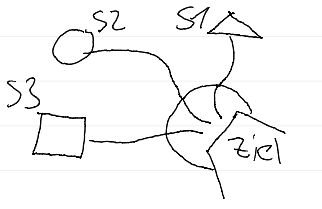
\includegraphics[width=1\linewidth]{content/pictures/Startplaces_Sketch.png}
\caption{Sketchzeichnung der Starträume (Quelle: eigene Darstellung)}
\label{fig:sketch-starterrooms}
\end{figure}

Der Watcher muss darüber hinaus erkennen können, welches Ziel in der Spielwelt als nächstes angesteuert werden soll. Um dies zu ermöglichen, muss die Gestaltung der Spielumgebung so ausfallen, dass entweder ein einzelnes oder mehrere klar identifizierbare Ziele vorhanden sind, auf die sich die Spieler gemeinsam zubewegen können. Für den ersten Abschnitt des Tutorials bietet es sich an, mit einem eindeutigen Ziel zu arbeiten, zu dem alle möglichen Wege führen. Dieses Ziel ist in der Skizze von Abbildung \ref{fig:sketch-starterrooms} deutlich erkennbar.

Zudem sollen die grundlegenden Mechaniken und Funktionen, die mit der Spielerrolle des Watchers einhergehen, erlernt werden. Dazu zählen insbesondere das Platzieren, Previewen und Entfernen von Gegenständen. Das Platzieren kann eingeleitet werden, indem der Watcher zu Beginn des Spiels bereits einen Gegenstand, bspw. eine Säule, im Inventar besitzt, für den lediglich ein geeigneter Platz in der Spielwelt gefunden werden muss. Ein weiteres Lernziel wird durch ein Hindernis umgesetzt, das dem Player nur noch ein passender Gegenstand, etwa eine Fackel, fehlt, um dieses zu überwinden. Diese Konstellation fordert den Watcher dazu auf, dem Player den benötigten Gegenstand aus dem Inventar bereitzustellen.

Das entfernen bereits platzierter Objekte kann wieder dadurch eingeführt werden, dass sich der Player im Zielbereich, die Eingangshalle (der Bereich, der an das Ziel angrenzt) aus Abbildung \ref{fig:sketch-starterrooms}, befindet und dort bspw. eine Tür zu einem neuen Abschnitt öffnen muss. Hierfür werden erneut jene Gegenstände benötigt, die bereits in den zwei vorherigen Rätseln verwendet wurden. Daraus ergibt sich die Notwendigkeit, zuvor platzierte Objekte aus der Spielwelt zu entfernen und diese an neuen Stellen erneut einzusetzen.


Darüber hinaus erlernt der Watcher die Spielwelt zu interpretieren. Dabei existieren gezielt eingebaute Unterschiede in der Darstellung der Spielwelt zwischen der Anwendung des Players und der des Watchers. Diese Inkonsistenzen sollen gezielt die Kommunikation zwischen beiden Rollen anregen und fördern. Dieser Aspekt wurde sich in der vorangegangenen Ausarbeitung im Feedback gewünscht. Konkret wird dies durch das Fehlen bestimmter Türen in den Startbereichen des Players oder an den Durchgängen zum Eingangsportal des nächstes Abschnitts realisiert.

Analog zum Watcher erhält auch der Player eine kurze Einführung in die grundlegenden Steuerungsmechaniken seiner Anwendung. Während sich die meisten Rätsel und Hindernisse innerhalb der Anwendungen des Players befinden, sind einige Interaktionen auch auf Seiten des Watchers verortet. Der Player muss daher in der Lage sein, relevante Rätsel, Hindernisse und Hinweise zu identifizieren und korrekt anzuwenden. Um den Einstieg in die Spielmechanik zu erleichtern, wird in den Starträumen des Players eine kleine Notiz platziert, die einen ersten Hinweis auf die Funktionsweise der Watcher-Mechaniken sowie auf das Lösen des ersten gemeinsamen Hindernisses gibt.

\begin{figure}[ht]
\centering
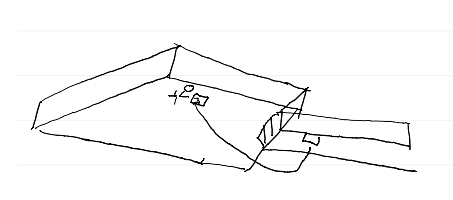
\includegraphics[width=1\linewidth]{content/pictures/Startroom_Sketch.png}
\caption{Sketchzeichnung des Hinweises für das erste Hindernis (Quelle: eigene Darstellung)}
\label{fig:sketch-startriddle}
\end{figure}

Abbildung \ref{fig:sketch-startriddle} zeigt eine erste konzeptionelle Überlegung, bei der eine im Startraum platzierte Notiz den Player darauf hinweist, dass ein schwerer Gegenstand auf eine Druckplatte gestellt werden muss, um die Tür zum angrenzenden Flur zu öffnen. Dieses Rätsel dient als Einführung in die Spielmechanik des indirekten Türöffnen und betont zugleich die Notwendigkeit der Kooperation zwischen Player und Watcher.

Darüber hinaus soll dieser erste Abschnitt das Tragen und Platzieren von Gegenständen vermitteln. Zu diesem Zweck kann ein weiteres Hindernis eingebaut werden, das bspw. durch das Einsetzen eines Objektes, wie einer Fackel in eine entsprechende Halterung, überwunden werden muss. In diesem Fall ist der Player auf die Unterstützung des Watchers angewiesen, der den benötigten Gegenstand auswählt und übermittelt. Der Player wiederum muss den Gegenstand korrekt einsetzen, um das Hindernis zu lösen.

Als letztes Lernziel in diesem Abschnitt wird das Freischalten neuer Bereiche eingeführt. Dieses Ziel betrifft sowohl den Player als auch den Watcher, da beide gemeinsam Bedingungen erfüllen müssen, um Zugang zu weiteren Abschnitten der Spielwelt zu erhalten.

\paragraph{Beschreibung des Abschnittes}

\begin{figure}[ht]
\centering
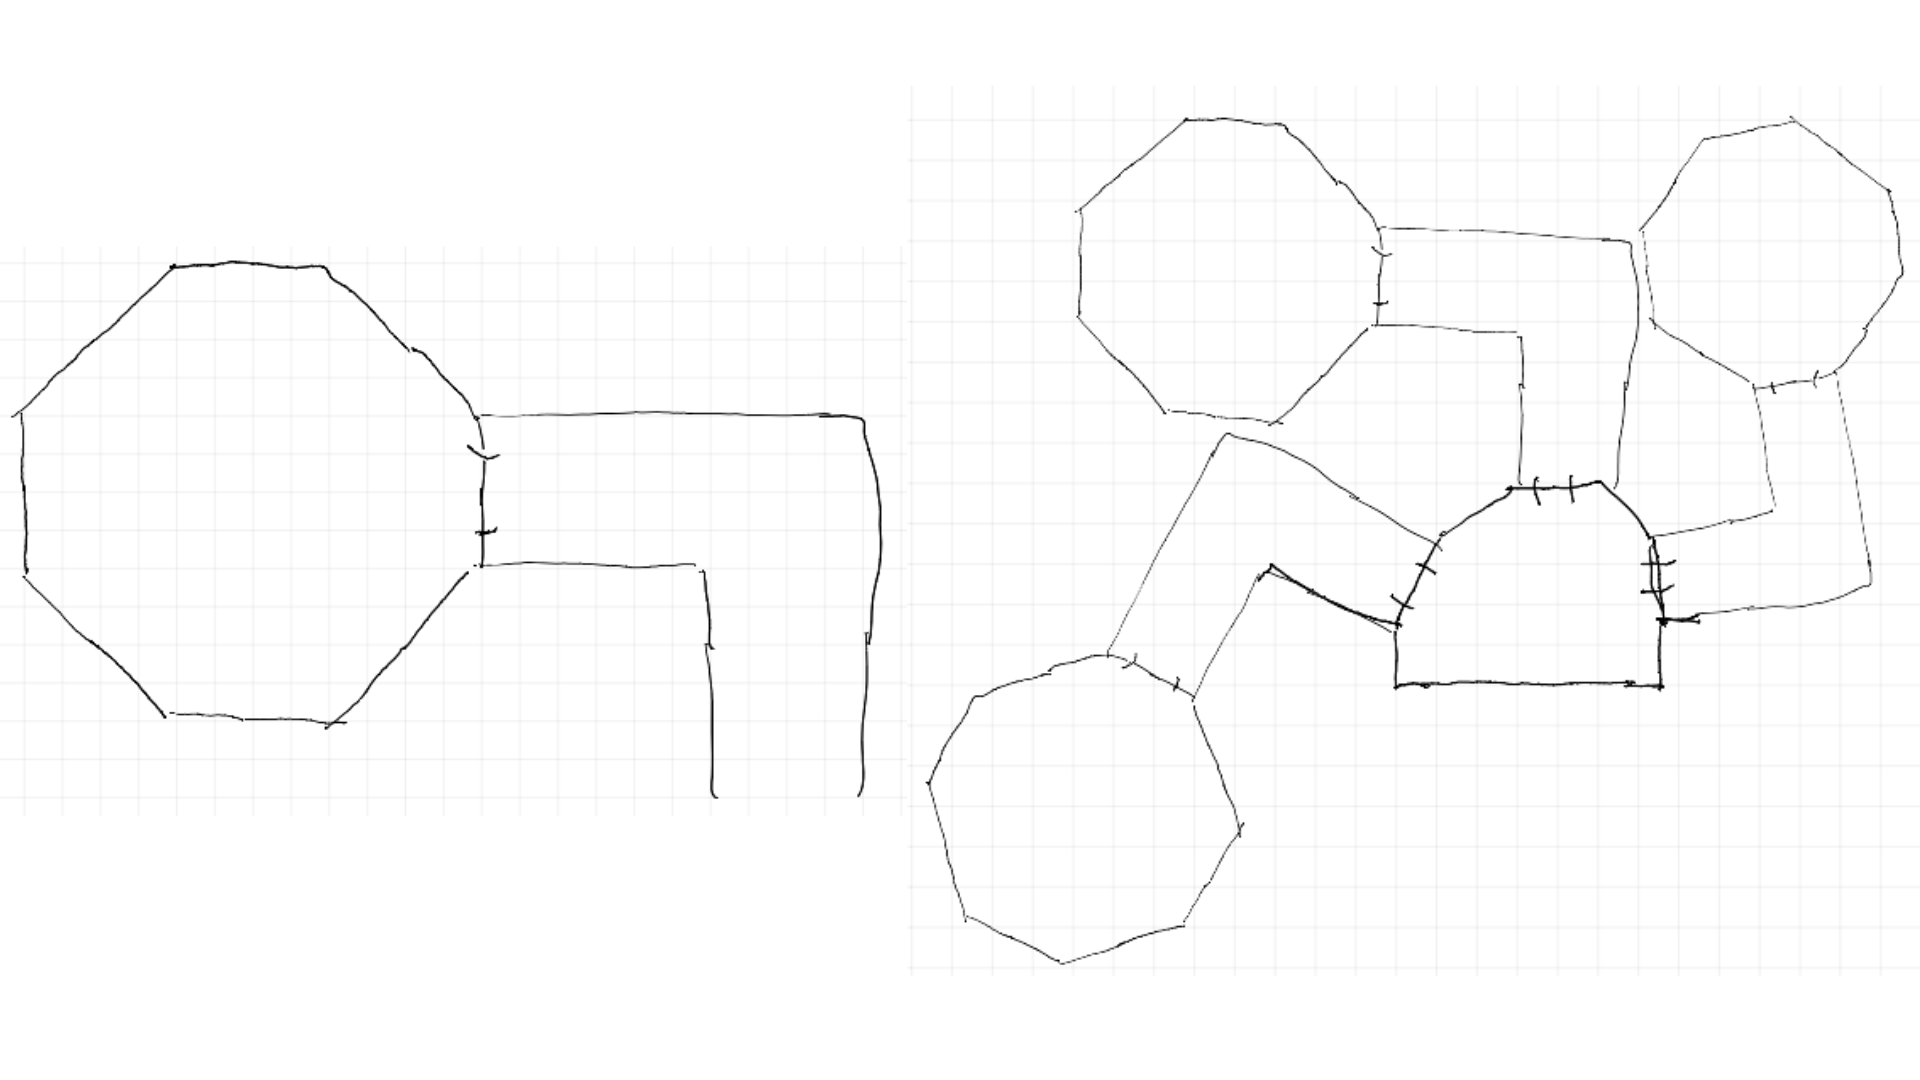
\includegraphics[width=1\linewidth]{content/pictures/Abschnitt_Concept_00.png}
\caption{Konzept Abschnitt 1 (Quelle: eigene Darstellung)}
\label{fig:section_00_concept}
\end{figure}

Abbildung \ref{fig:section_00_concept} zeigt eine erste Konzeptzeichnung des Einstiegsabschnitts. Auf der linken Seite ist ein sechseckiger Raum dargestellt, in dem der Spieleravatar des Players zu Beginn der Spielsequenz platziert wird. Dieser Startbereich existiert, wie auf der rechten Seite der Abbildung zu erkennen ist, in drei Varianten. Der Player muss seinem Watcher mitteilen, in welchem der drei Räume er sich befindet. Dies erfordert eine gezielte Beschreibung der Umgebung und stellt somit eine erste kommunikative Aufgabe dar.

Die Unterscheidung der Räume erfolgt über visuelle Merkmale in deren Gestaltung. Wie in Abbildung \ref{fig:corridors} dargestellt, besitzt der erste Raum (erste Reihe, linkes Bild) einen zentral angebrachten Kronleuchter, der zweite Raum (zweite Reihe, linkes Bild) ist durch einen großflächigen Teppich gekennzeichnet, während sich im dritten Raum (dritte Reihe, linkes Bild) eine Bank zwischen zwei Innensäulen befindet. Diese unterschiedlichen Merkmale dienen als Referenzpunkte für die verbale Orientierung und fördern die Koordination zwischen beiden Rollen zu Spielbeginn.

\begin{figure}[ht]
\centering
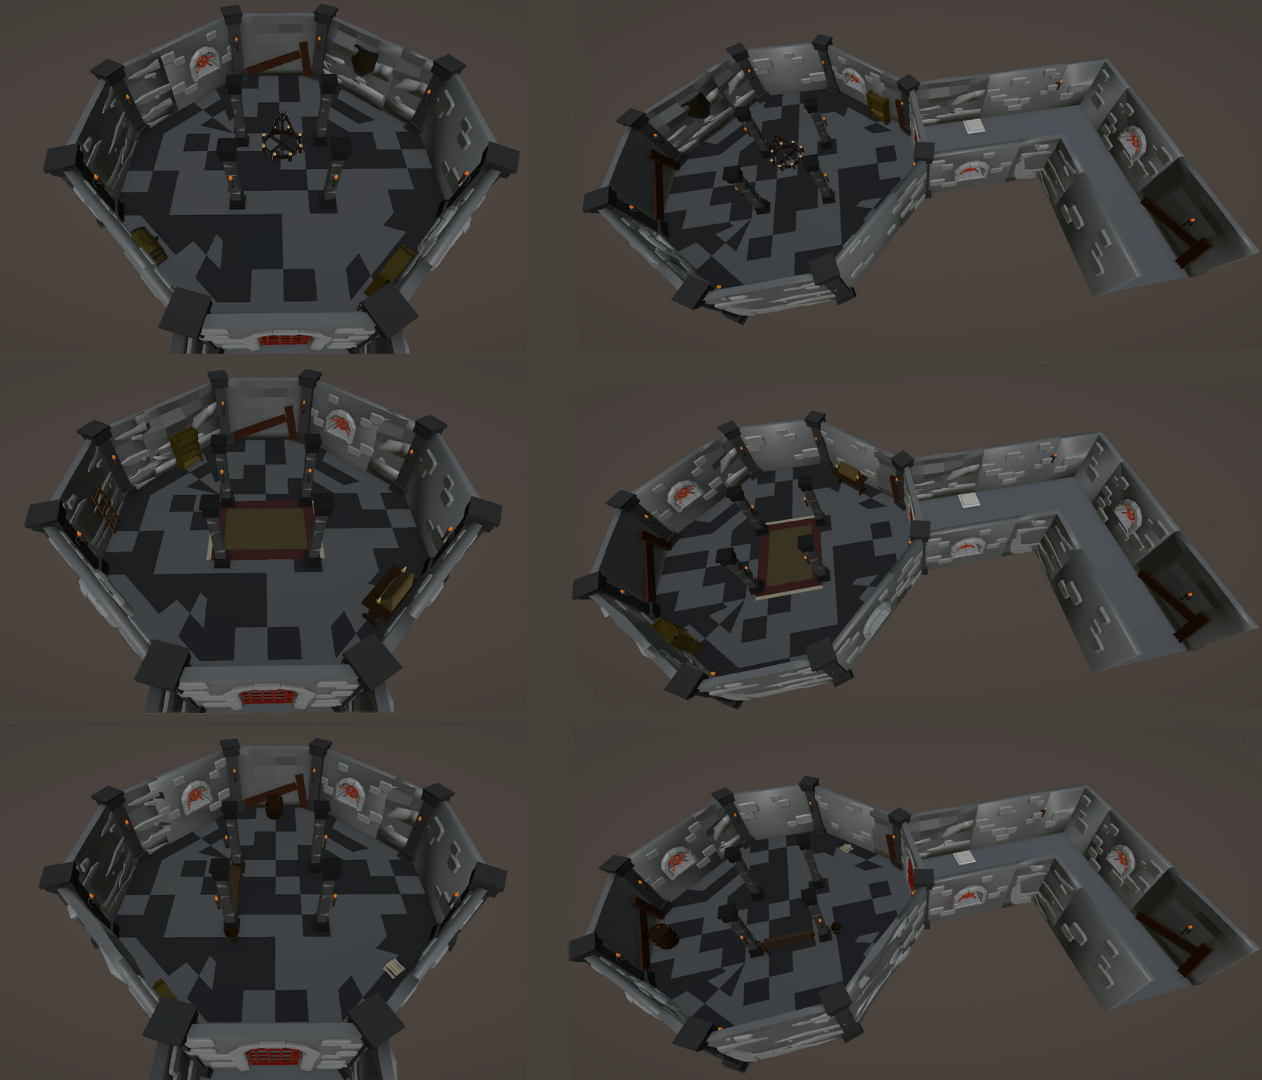
\includegraphics[width=1\linewidth]{content/pictures/Room_00-Room_02-Corridor_00-Corridor_02.png}
\caption{Korridor 1 bis Korridor 3 (Quelle: eigene Darstellung)}
\label{fig:corridors}
\end{figure}

Wie auf der rechten Darstellung der Konzeptzeichnung in Abbildung \ref{fig:section_00_concept} ersichtlich, führen die drei Starträume jeweils über einen Flur in eine zentrale Eingangshalle. Diese architektonische Verbindung ist in Abbildung \ref{fig:section_00} visualisiert. An der gegenüberliegenden Wand der Flure befindet sich eine verschlossene Tür, die vom Player, in Zusammenarbeit mit dem Watcher, geöffnet werden muss, um den Zugang zum nächsten Spielabschnitt zu ermöglichen.

\begin{figure}[ht]
\centering
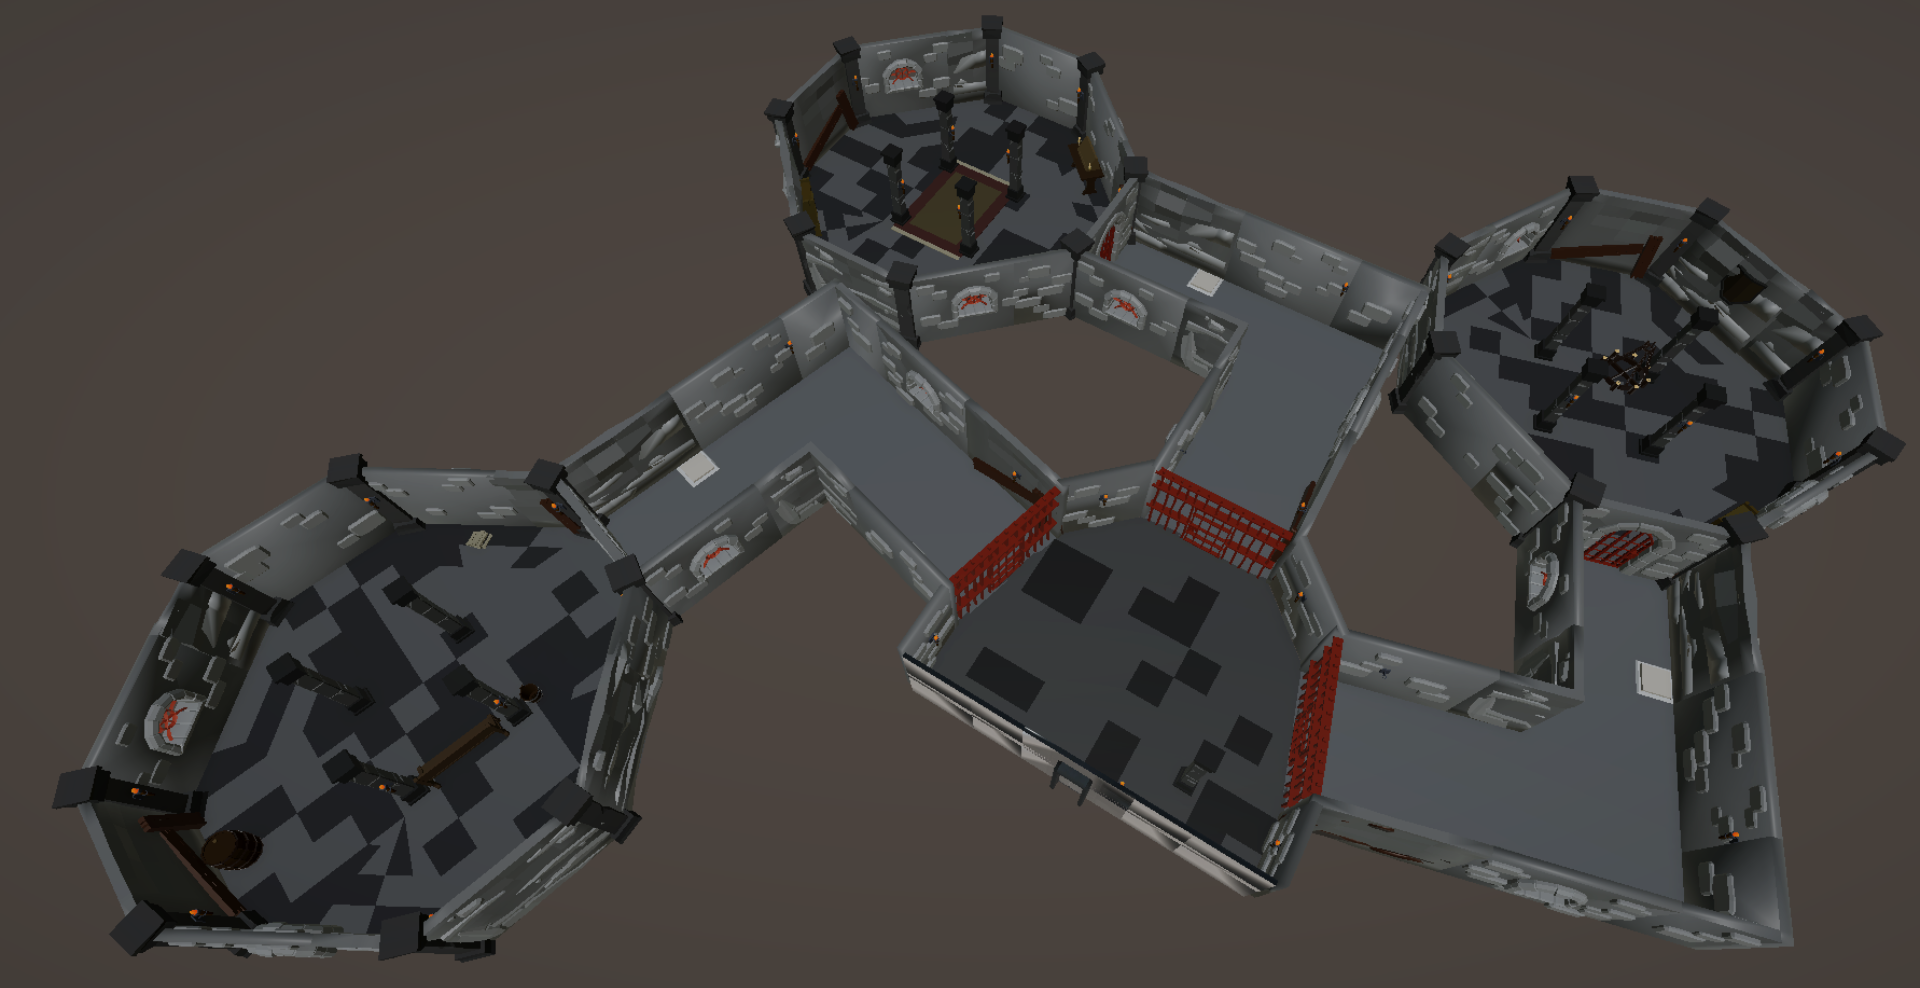
\includegraphics[width=1\linewidth]{content/pictures/Abschnitt_00.PNG}
\caption{Abschnitt 1 (Quelle: eigene Darstellung)}
\label{fig:section_00}
\end{figure}

Zu Beginn erhält der Watcher eine Übersicht über den gesamten ersten Spielabschnitt, wie in Abbildung \ref{fig:section_00} dargestellt. Im Gegensatz dazu ist das Sichtfeld des Players zu Beginn auf einen der drei Starträume (vgl. Abbildung \ref{fig:corridors}) sowie den angrenzenden Flur beschränkt. Die beiden übrigen Starträume sowie deren zugehörige Flure bleiben für den Player dauerhaft unzugänglich, auch nachdem er die Eingangshalle zum nächsten Abschnitt betreten hat.

\subsection{Abschnitt 2: Der Sicherheitsraum}

Analog zum ersten Abschnitt werden zunächst die zugrunde liegenden Lernziele sowie die konzeptionellen Überlegungen erläutert, bevor im Anschluss der Aufbau des Abschnitts im Detail vorgestellt wird.

\paragraph{Lernaspekte und Konzeption dieses Abschnittes}

Im zweiten Abschnitt lernt der Watcher, das ihm neue Räume angezeigt werden können (die dem Player verborgen bleiben), sobald diese vom Player freigeschaltet wurden. Der Player kann bspw. einen Mechanismus aktivieren, durch den ein bislang verborgener Bereich sichtbar wird, in welchem der Watcher anschließend ein Rätsel lösen muss.

Darüber hinaus erkennt der Watcher neu entdeckte Objekte, die der Player in der Spielwelt gefunden hat, als platzierte Gegenstände. Diese Objekte kann der Watcher bei Bedarf wieder entfernen. Solche Gegenstände können bspw. zur Lösung weiterer Aufgaben genutzt werden.

In diesem Zusammenhang erlernt der Player das gezielte Entdecken von Gegenständen, etwas durch das Vorbeigehen in unmittelbarer Nähe. Technisch kann dies so umgesetzt werden, dass beim Annähern ein Tooltip eingeblendet wird und der Gegenstand dadurch auch für den Watcher sichtbar wird.

\paragraph{Beschreibung des Abschnittes}

\begin{figure}[ht]
\centering
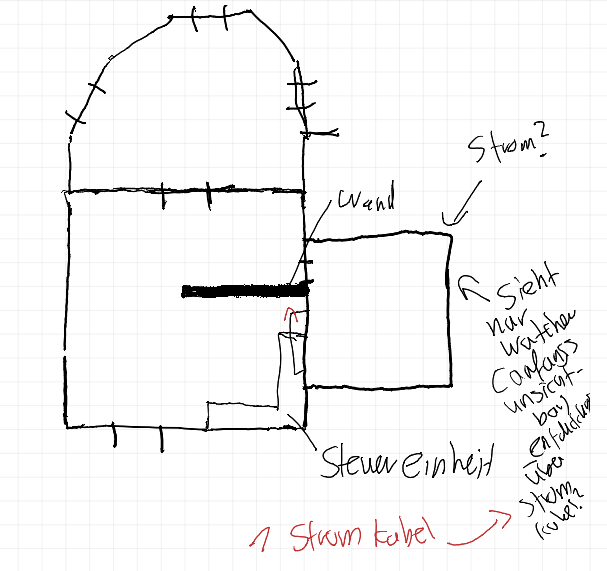
\includegraphics[width=1\linewidth]{content/pictures/Abschnitt_Concept_01.PNG}
\caption{Konzept Abschnitt 2 (Quelle: eigene Darstellung)}
\label{fig:section_01_concept}
\end{figure}

Abbildung \ref{fig:section_01_concept} zeigt eine erste Konzeptzeichnung des zweiten Abschnitts, der als Sicherheitsraum konzipiert ist. Dieser Abschnitt fungiert als verbindendes Element zwischen dem zuvor beschriebenen Startraum und dem nachfolgendem Bereich in Abschnitt drei. Der Player betritt den Sicherheitsraum über den oberen Zugang, der von der Eingangshalle aus erreichbar ist.

Der Raum verfügt auf der rechten Seite über eine Tür, die zu einem Innenhof bzw. einem Außenbereich führt. Über den unteren Ausgang kann ein weiterer Abschnitt betreten werden. Zentral für die Funktion dieses Raumes als Sicherheitsbereich ist ein Überwachungsterminal, das sich in der unteren rechten Ecke befindet.

Um die im Sicherheitsraum tätigen Personen vor Einblicken oder Störungen durch andere Mitarbeiter oder Spielcharaktere abzuschirmen, wurde zwischen dem Terminal und der rechten Tür eine Trennwand vorgesehen.

\begin{figure}[ht]
\centering
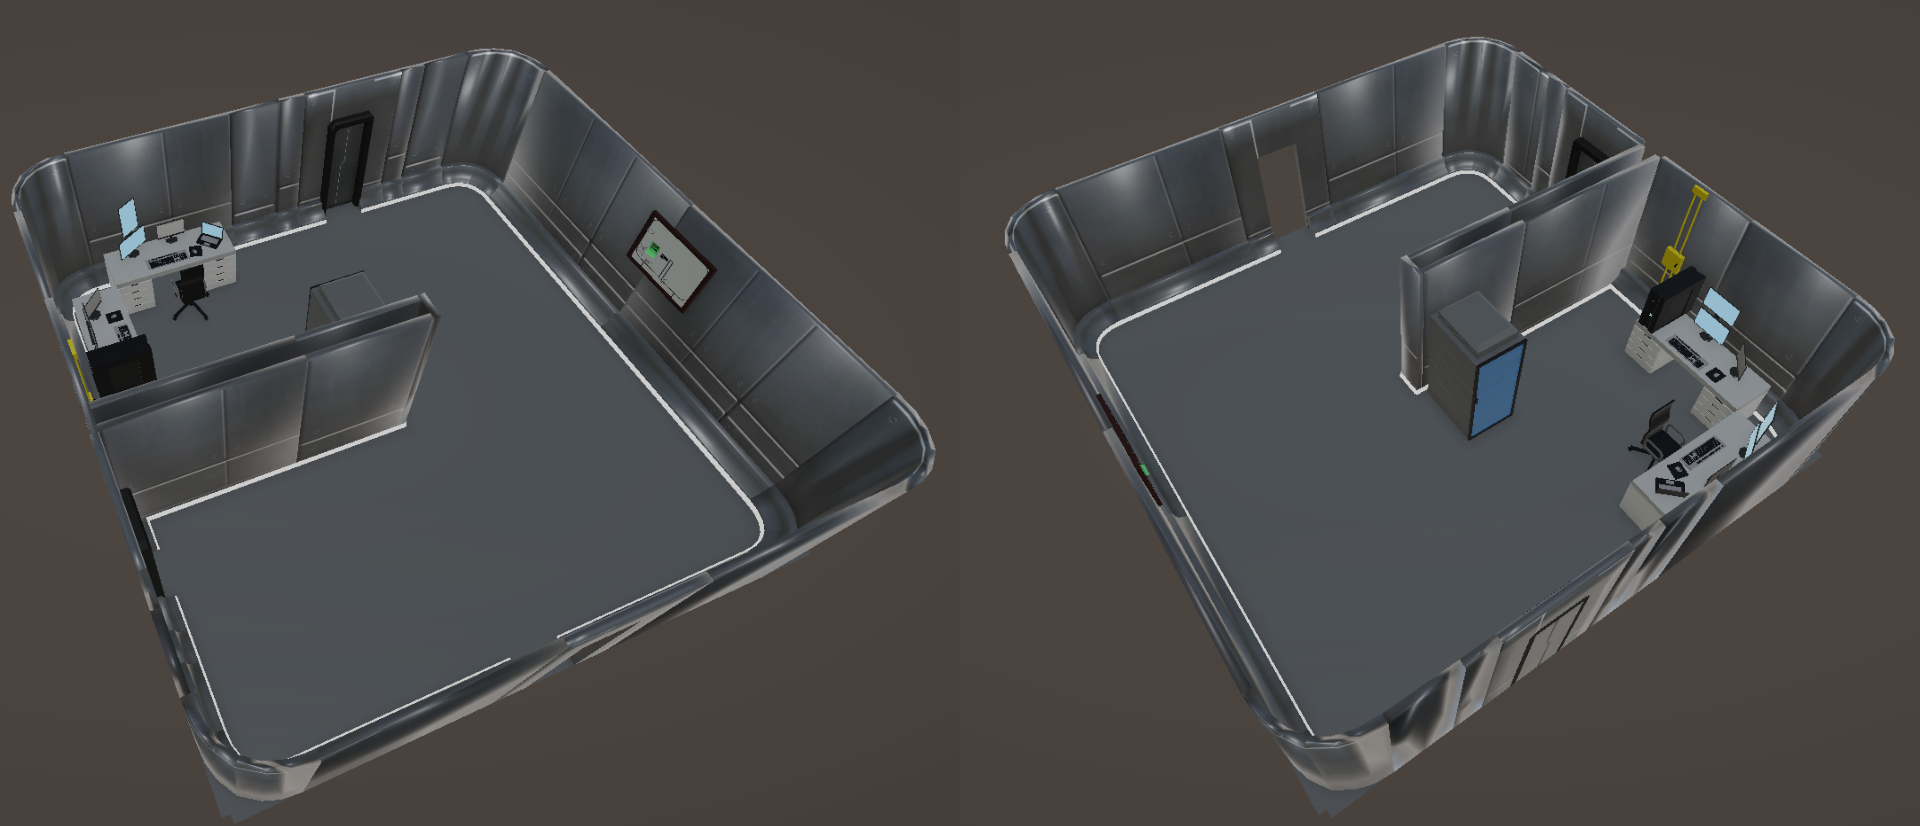
\includegraphics[width=1\linewidth]{content/pictures/Abschnitt_01 - Player.png}
\caption{Abschnitt 2 aus Sicht des Players (Quelle: eigene Darstellung)}
\label{fig:section_01_player}
\end{figure}

\begin{figure}[ht]
\centering
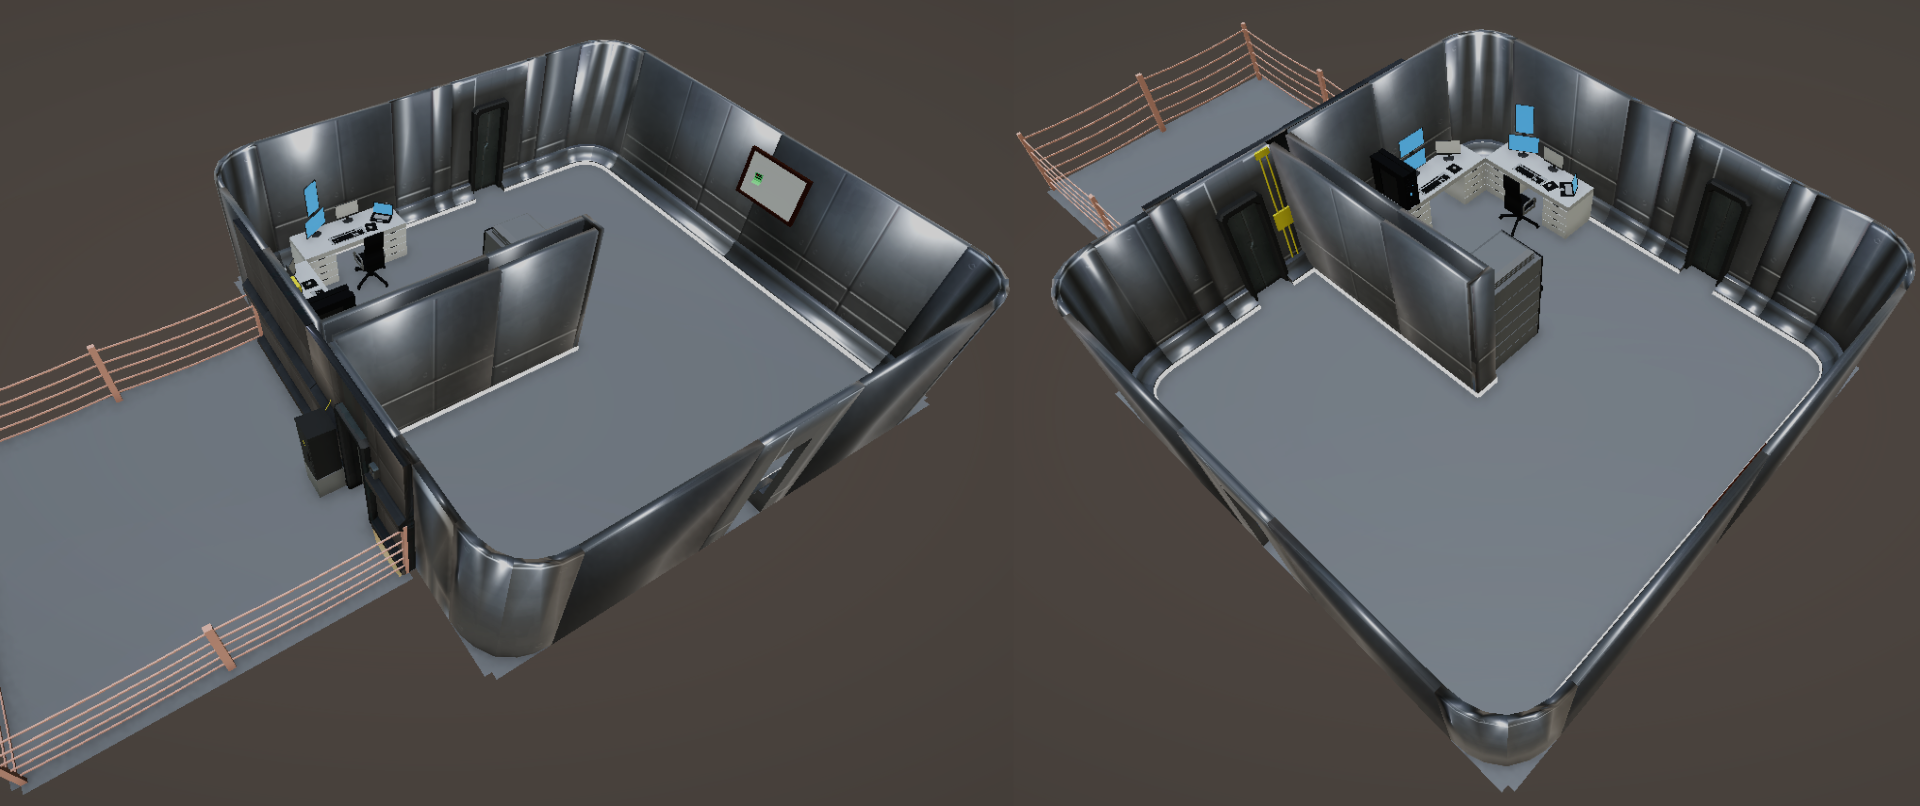
\includegraphics[width=1\linewidth]{content/pictures/Abschnitt_01 - Watcher.png}
\caption{Abschnitt 2 aus Sicht des Watchers (Quelle: eigene Darstellung)}
\label{fig:section_01_watcher}
\end{figure}

Die Abbildungen \ref{fig:section_01_player} und \ref{fig:section_01_watcher} zeigen den Sicherheitsraum aus den jeweiligen Perspektiven von Player und Watcher. Die gezielten Unterschiede in der visuellen Gestaltung der beiden Szenen zielen darauf ab, eine intensivere verbale Abstimmung zwischen den Spielerrollen zu fördern. Beide Versionen des Raumes enthalten einen gelben Sicherungskasten, zu dem gelbe Leitungen führen und von dem sie auch wieder wegführen.

In der Player-Ansicht (vgl. Abbildung \ref{fig:section_01_player}) befindet sich der Sicherungskasten im rechten Bild links neben dem PC an der Rückwand zum Außenbereich. In der Watcher-Ansicht (vgl. Abbildung \ref{fig:section_01_watcher}) ist er hingegen rechts neben der Tür zum Außenbereich positioniert. Auf der Rückseite des Sicherungskasten befindet sich ein Stromgenerator, der nur in der Watcher-Ansicht sichtbar ist, dort ist er links neben der Tür zum Außenbereich zu erkennen. In der Anwendung des Players fehlt dieser Stromgenerator vollständig.

Dieser asymmetrische Informationszugang ist zentral für das im Raum enthaltene Rätsel. Nur der Watcher kann den Außenbereich mit dem Generator sehen und muss mithilfe der vom Player bereitgestellten Informationen eigenständig zur Lösung gelangen. Die Raumgestaltung unterstützt somit gezielt eine wechselseitige Abhängigkeit beider Rollen in der Kommunikation und Interaktion.

\subsection{Abschnitt 3: Das Büro}

Der dritte Abschnitt fungiert im Rahmen des Tutorials nicht mehr als expliziter Lernbereich, sondern dient vielmehr als Anwendungsumgebung für die zuvor erlernten Mechaniken. Als szenisches Setting wurde ein Bürotrakt innerhalb eines größeren Bürokomplexes gewählt, welcher zugleich Teil der Spielumgebung in der Haupthandlung ist. Der zuvor durchlaufene Abschnitt hatte die Funktion eines Kontrollraums und stellt die Verbindung zwischen dem Anfangsbereich und dem Bürokomplex her.

\begin{figure}[ht]
\centering
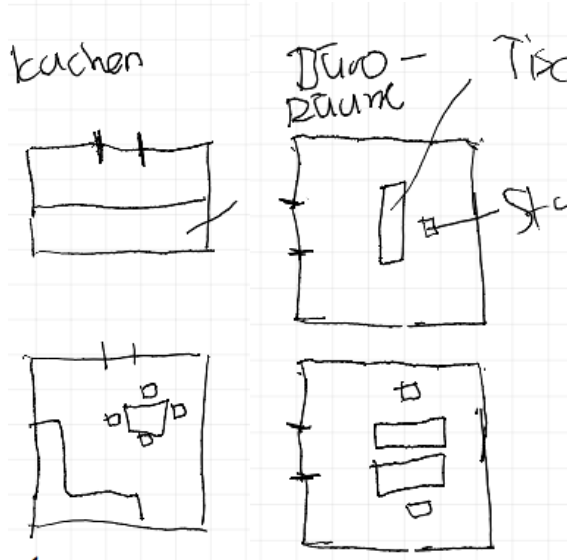
\includegraphics[width=0.6\linewidth]{content/pictures/Abschnitt_02_Concept.png}
\caption{Konzept Abschnitt 3 (Quelle: eigene Darstellung)}
\label{fig:section_02_concept}
\end{figure}

Abbildung \ref{fig:section_02_concept} zeigt erste konzeptionelle Überlegungen zur räumlichen Gestaltung innerhalb des Bürokomplexes, die in Abbildung \ref{fig:section_02} weiter ausgearbeitet und ergänzt wurden.

\begin{figure}[ht]
\centering
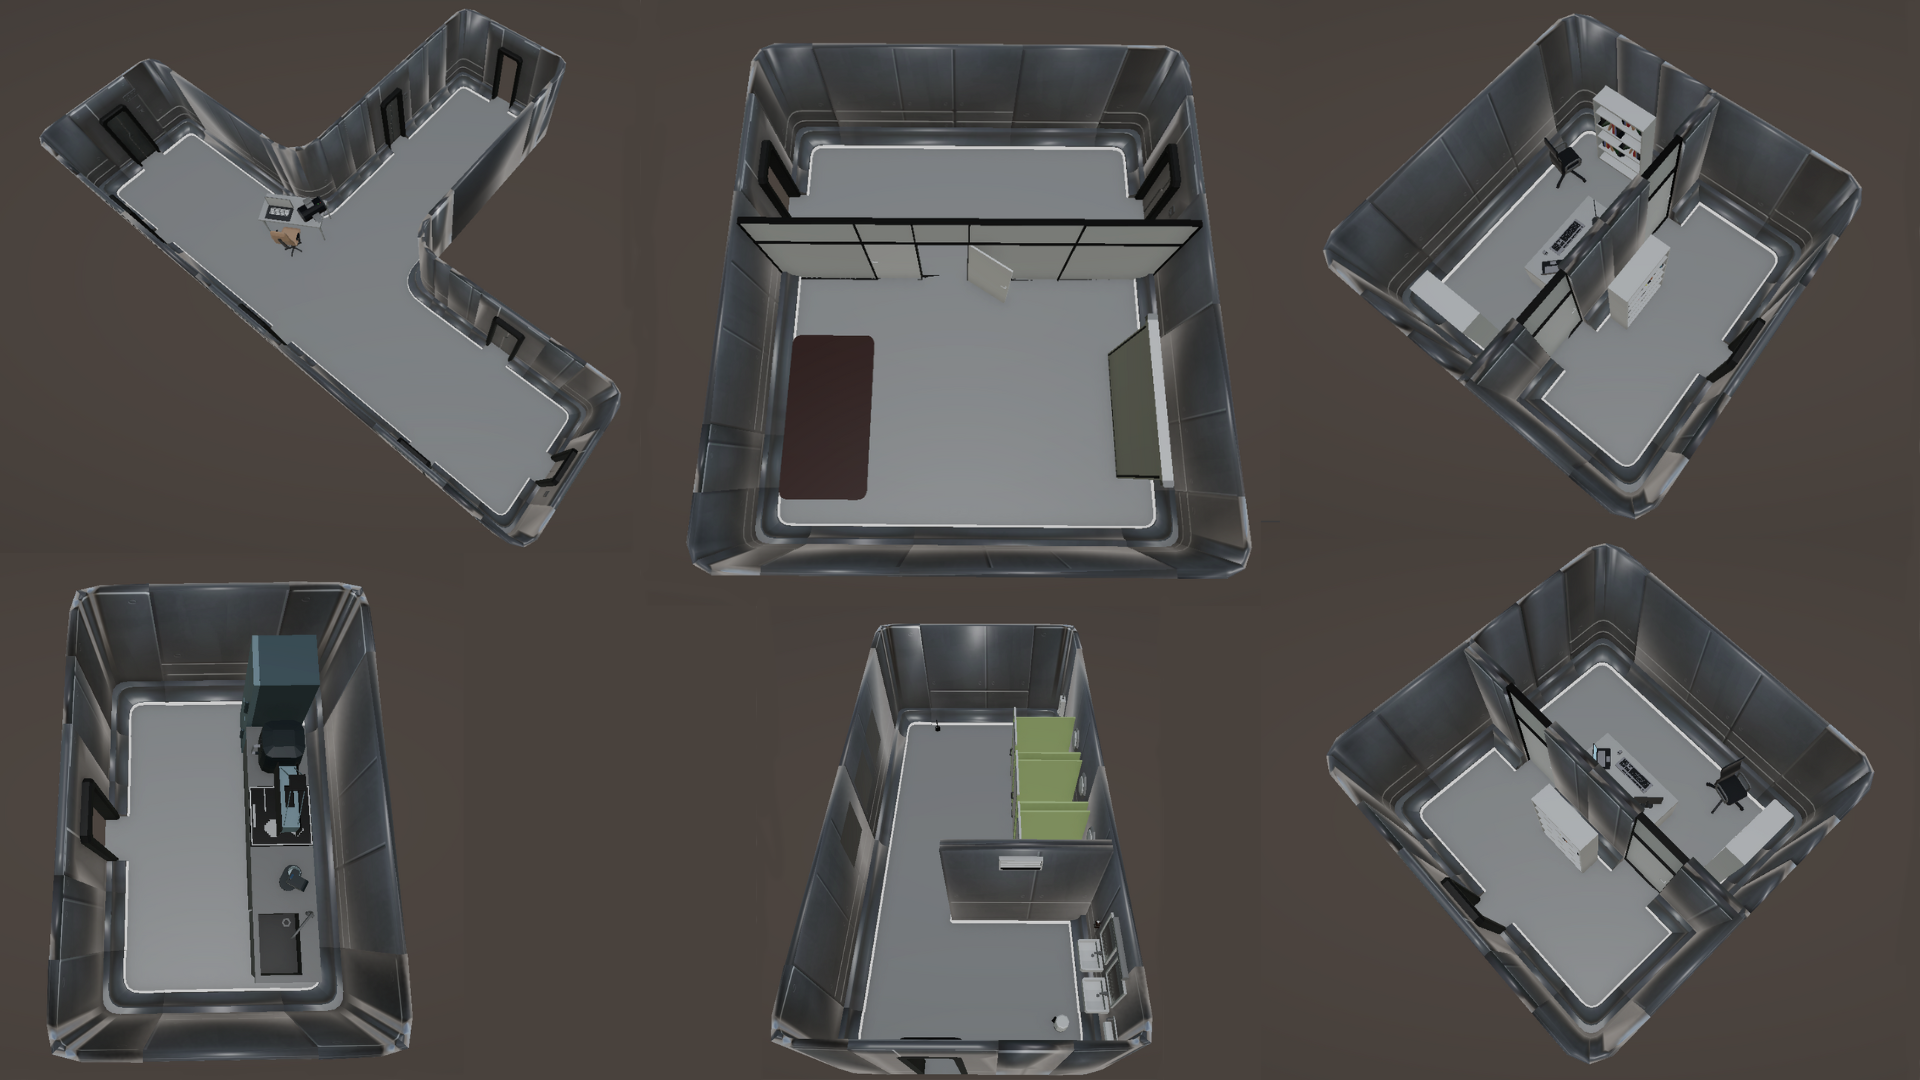
\includegraphics[width=1\linewidth]{content/pictures/Abschnitt_02.png}
\caption{Abschnitt 3 (Quelle: eigene Darstellung)}
\label{fig:section_02}
\end{figure}

Der Bürokomplex im letzten Abschnitt des Tutorials setzt sich aus mehreren Räumlichkeiten zusammen, in Abbildung \ref{fig:section_02} zu sehen. Einem Korridor (oben links in der Abbildung), einer Küche (unten links), einem Tagungsraum (oben mittig), einem kleinen WC (unten mittig), sowie zwei Büros (oben und unten rechts). Auch in diesem Bereich bestehen Unterschiede in der Wahrnehmung zwischen der Anwendung des Players und der des Watchers. Beide sehen jeweils nur eines der beiden Büros, die zueinander gespiegelt angelegt sind. Jedes dieser Büros beinhaltet ein separates Rätsel, sowie Hinweise darauf, wie nach dessen Lösung fortgefahren werden kann.

In der Player-Ansicht befinden sich im Tagungsraum zudem mehrere Stühle, die zunächst entdeckt werden müssen, bevor sie dem Watcher als Objekte zur Verfügung stehen. Die funktionale Einbindung dieser Räume und ihr Beitrag zum Gesamtpuzzle werden im folgenden Kapitel \emph{\nameref{sec:riddles}} näher erläutert.

\subsection{Rätseldesign}\label{sec:riddles}

Der Aufbau der Rätsel in den Abschnitten 1 und 2 folgt einer linearen Struktur, da sie primär der Einführung in die grundlegenden Spielmechaniken dienen. Die zugehörigen Hinweise sind in der Regel räumlich nah am jeweiligen Rätsel platziert. Entweder direkt in die Umgebung oder in Form von Notizen integriert.

\paragraph{Abschnitt 1}

\begin{figure}[ht]
\centering
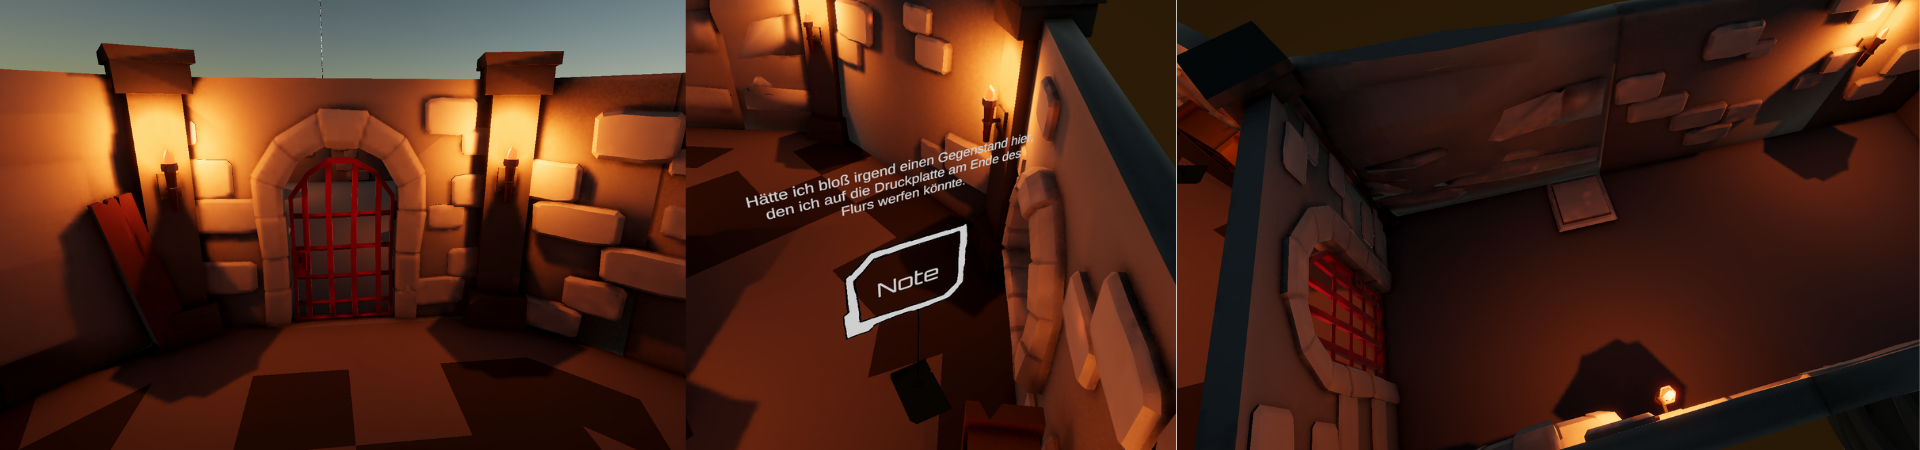
\includegraphics[width=1\linewidth]{content/pictures/Rätseldesign - Abschnitt00 - Rätsel00.png}
\caption{Aufbau der Rätsel von Abschnitt 1, Teil 1 (Quelle: eigene Darstellung)}
\label{fig:riddle-design-section00-00}
\end{figure}

\begin{figure}[ht]
\centering
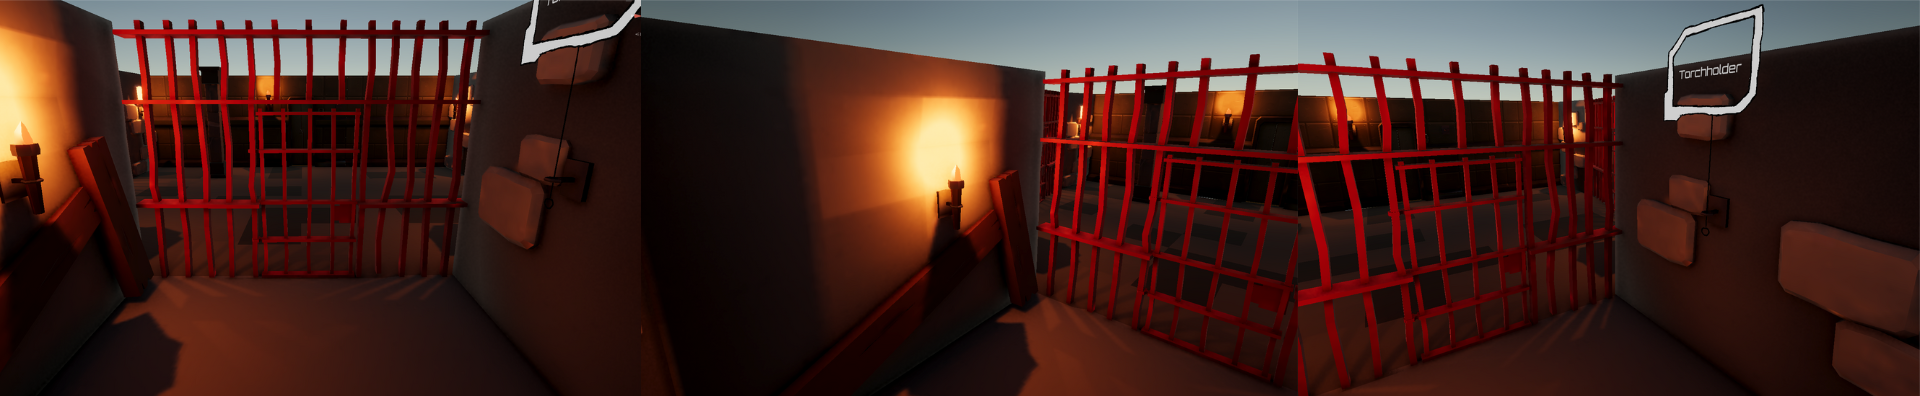
\includegraphics[width=1\linewidth]{content/pictures/Rätseldesign - Abschnitt00 - Rätsel01.png}
\caption{Aufbau der Rätsel von Abschnitt 1, Teil 2 (Quelle: eigene Darstellung)}
\label{fig:riddle-design-section00-01}
\end{figure}

\begin{figure}[ht]
\centering
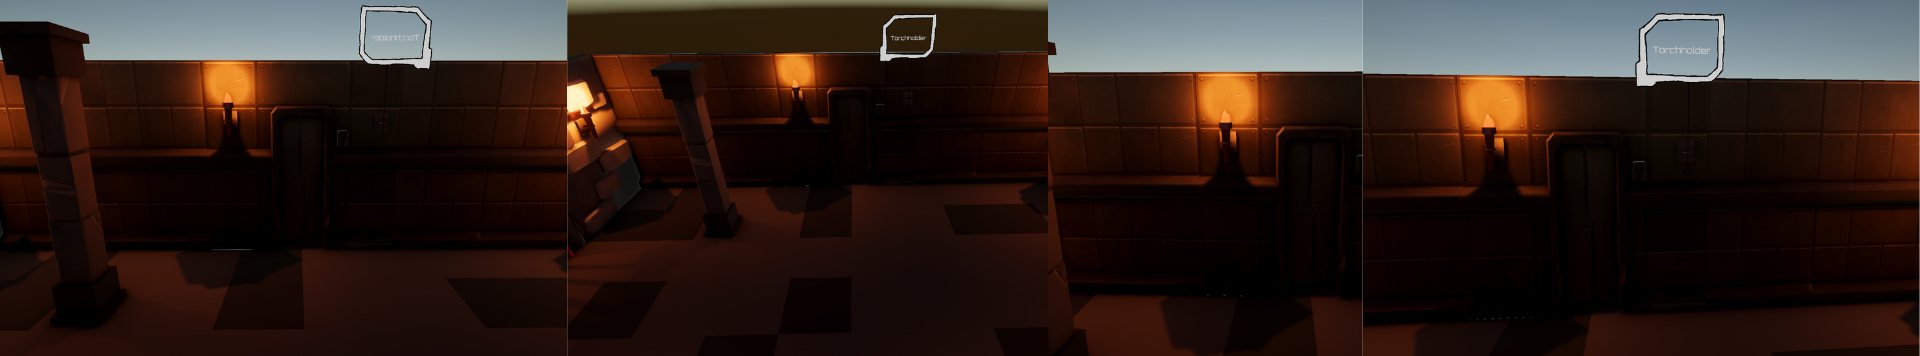
\includegraphics[width=1\linewidth]{content/pictures/Rätseldesign - Abschnitt00 - Rätsel02.png}
\caption{Aufbau der Rätsel von Abschnitt 1, Teil 3 (Quelle: eigene Darstellung)}
\label{fig:riddle-design-section00-02}
\end{figure}

Zu Beginn befindet sich der Player innerhalb eines Verlieses. Eine verrostete Eisentür blockiert den Weg aus diesem Raum (vgl. Abbildung \ref{fig:riddle-design-section00-00}, linkes Bild). Auf einer Notiz (vgl. Abbildung \ref{fig:riddle-design-section00-00}, mittleres Bild) erhält der Player den Hinweis, einen Gegenstand auf eine Druckplatte zu werfen (vgl. Abbildung \ref{fig:riddle-design-section00-00}, rechtes Bild). Gemeint ist damit das Platzieren eines schweren Gegenstandes, die verfügbare Säule die sich zu Spielbeginn im Inventar des Watchers befindet.

Nach dem Verlassen des Verlieses trifft der Player auf eine weitere verrostete Eisentür, die ebenfalls geöffnet werden muss (vgl. Abbildung \ref{fig:riddle-design-section00-01}, linkes Bild). An der linken Wandseite der Tür befindet sich eine Fackelhalterung mit einer eingesetzt Fackel, die sowohl vom Player als auch vom Watcher wahrgenommen wird (vgl. Abbildung \ref{fig:riddle-design-section00-01}, mittlere Bild). Auf der gegenüberliegenden Wandseite erkennen beide eine leere Fackelhalterung (vgl. Abbildung \ref{fig:riddle-design-section00-01}, rechts Bild). Aus dieser Konstellation ergibt sich die Schlussfolgerung, dass der Watcher dem Player eine Fackel senden muss, damit dieser sie in die leere Haltung einsetzt.

In der darauffolgenden Eingangshalle treffen beide Spieler auf eine verschlossene Sicherheitstür, die zum Abschluss des Abschnitts geöffnet werden muss (vgl. Abbildung \ref{fig:riddle-design-section00-02}, linkes Bild). Links von der Tür befinden sich eine Säule, sowie eine Fackelhalterung mit eingesetzter Fackel (vgl. Abbildung \ref{fig:riddle-design-section00-02}). Auf der rechten Seite ist eine weitere, leere Fackelhalterung zu sehen (vgl. Abbildung \ref{fig:riddle-design-section00-02}, rechts Bild). Die zuvor benutzte Fackel muss nun durch den Player in diese leere Halterung eingesetzt werden.

Darüber hinaus muss der Watcher die im ersten Rätsel verwendeten Säule gemäß der beiliegenden Beschreibung (\say{The column is required to match a pattern or to serve as a counterweight}) auf der gegenüberliegenden Seite der Tür so positionieren, dass beide Säulen symmetrisch zur Tür ausgerichtet sind (vgl. Abbildung \ref{fig:riddle-design-section00-02}, linkes Bild).

\paragraph{Abschnitt 2}

Abschnitt zwei setzt das lineare Rätseldesign aus dem ersten Abschnitt fort, wodurch die Spieler weiterhin schrittweise an die zugrunde liegenden Mechaniken herangeführt werden.

\begin{figure}[ht]
\centering
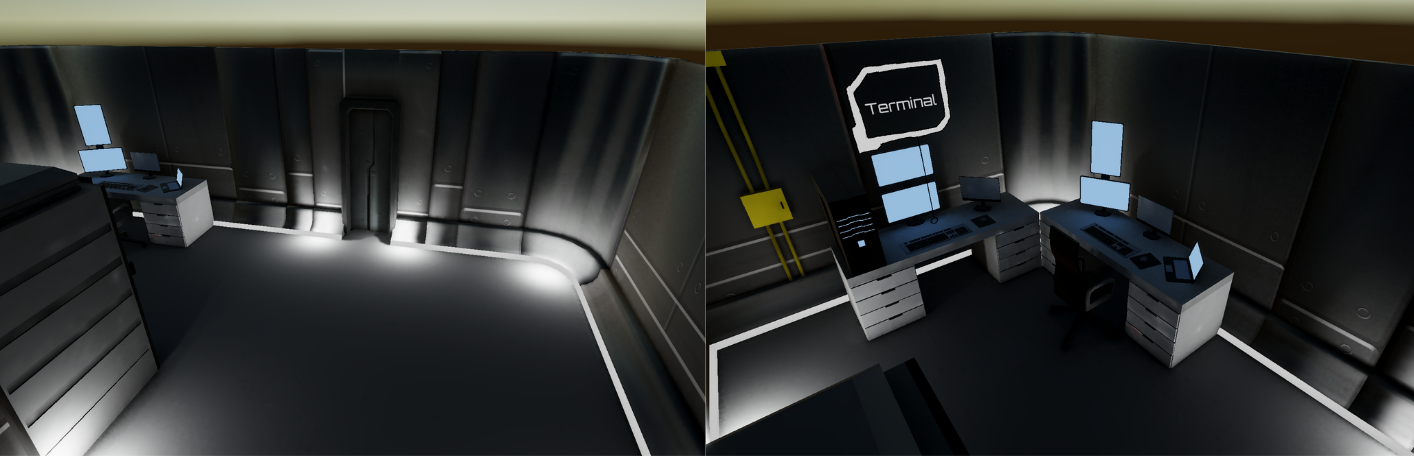
\includegraphics[width=1\linewidth]{content/pictures/Rätseldesign - Abschnitt01 - Rätsel00.png}
\caption{Aufbau der Rätsel von Abschnitt 2, Teil 1 (Quelle: eigene Darstellung)}
\label{fig:riddle-design-section01-00}
\end{figure}

\begin{figure}[ht]
\centering
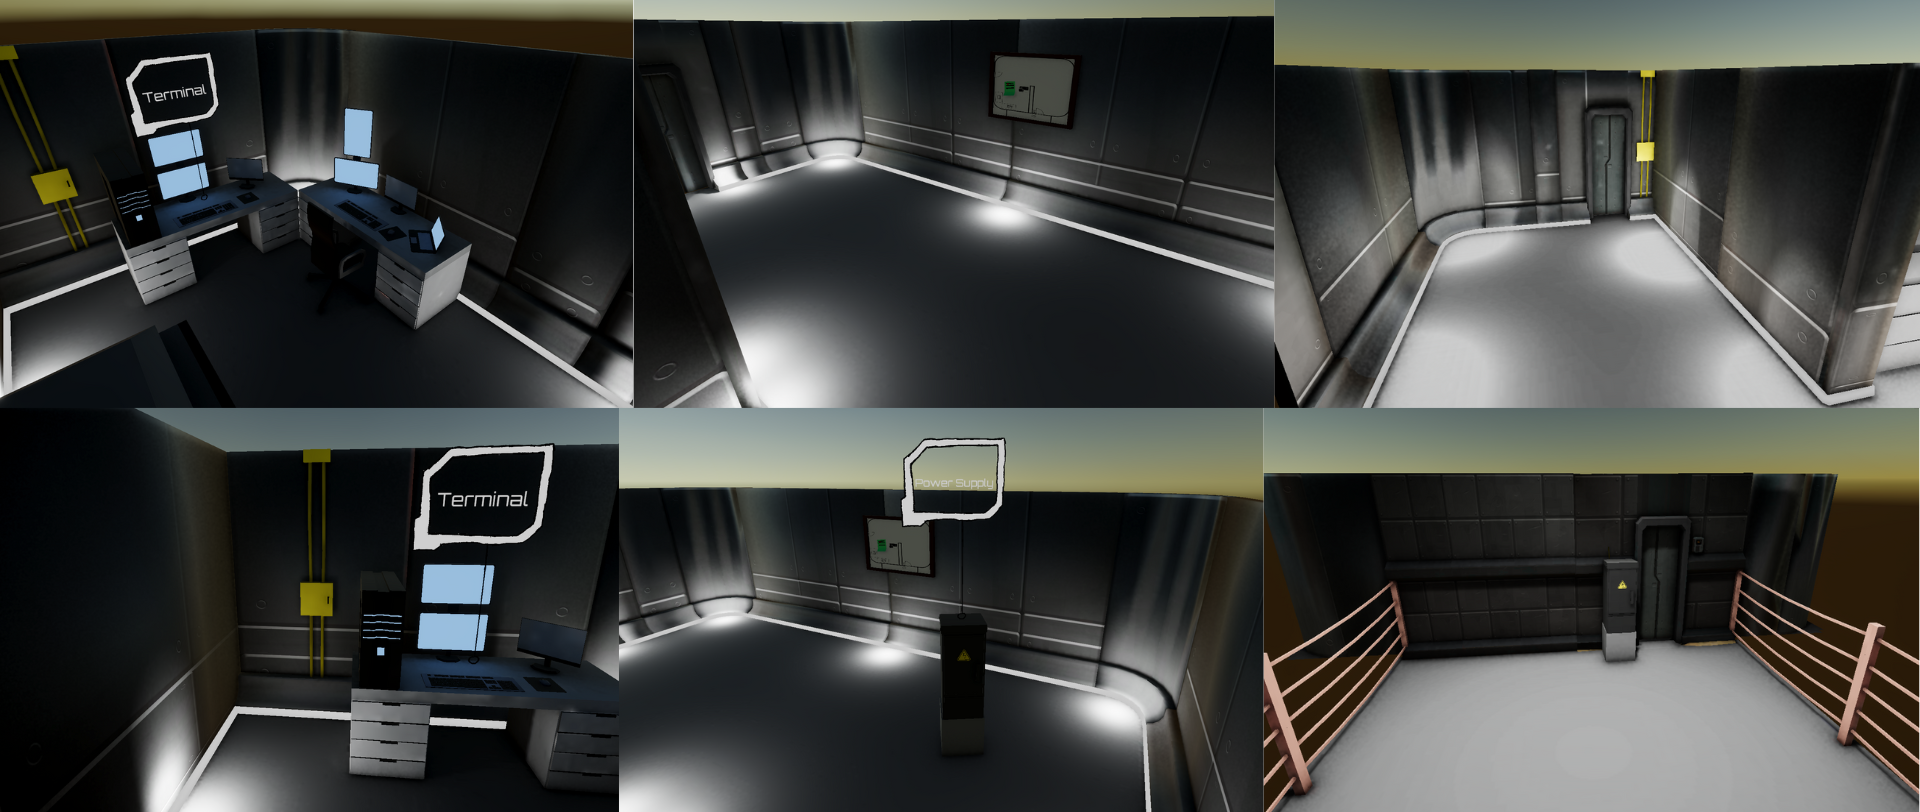
\includegraphics[width=1\linewidth]{content/pictures/Rätseldesign - Abschnitt01 - Rätsel01.png}
\caption{Aufbau der Rätsel von Abschnitt 2, Teil 2 (Quelle: eigene Darstellung)}
\label{fig:riddle-design-section01-01}
\end{figure}

Nachdem der Player den Sicherheitsraum betreten hat, trifft er auf zwei Türen. Eine befindet sich links vom Eingang, die andere liegt direkt gegenüber. Letztere markiert den Ausgang aus diesem Abschnitt, ist jedoch zu Beginn nicht passierbar, da der zugehörige Bewegungsmelder deaktiviert ist und zunächst aktiviert werden muss. Das dafür vorgesehen Terminal befindet sich links neben dem Ausgang (vgl. Abbildung \ref{fig:riddle-design-section01-00}), ist allerdings ohne Strom.

Sowohl der Player als auch der Watcher erhalten Hinweise darauf, wie die Stromversorgung für das Terminal wiederhergestellt werden kann. Innerhalb des Sicherheitsraums befindet sich ein Stromgenerator (vgl. Abbildung \ref{fig:riddle-design-section01-01}, Bild zweite Zeile Mitte), der an einer bestimmten Stelle positioniert werden muss. In der Ansicht des Watchers ist rechts neben der zweiten Tür im Sicherheitsraum, also der Tür, die sich vom Eingang aus links befindet, eine Sicherung zu sehen. Auf deren gegenüberliegender Seite befindet sich ein kleiner Innenhof, in dem ein weiterer Stromgenerator neben der Tür steht (vgl. Abbildung \ref{fig:riddle-design-section01-01}, Bilder erste und zweite Zeile rechts).

Der Player wiederum findet in seiner Version des Raumes einen Plan auf einer Pinnwand (vgl. Abbildung \ref{fig:riddle-design-section01-01}, Bild erste Reihe Mitte), der die Stromversorgung der Watcher-Anwendung darstellt. Ein zentraler Unterschied zwischen beiden Versionen besteht darin, dass sich die Sicherung in der Sicht des Players nicht neben der Tür, sondern links neben dem Terminal befindet (vgl. Abbildung \ref{fig:riddle-design-section01-01}, Bild zweite reihe links). Daraus ergibt sich, dass der Generator, ausgehend von der Ansicht des Watchers, auf der gegenüberliegenden Seite, also links neben dem bestehenden Stromkasten (vgl. Abbildung \ref{fig:riddle-design-section01-01}, Bild zweite Reihe rechts), platziert werden muss.

Sobald der Generator korrekt positioniert ist, lasst sich der Bewegungsmelder am Terminal aktivieren. Dadurch öffnet sich die Tür und die Spieler können Abschnitt drei betreten.

\paragraph{Abschnitt 3}

Abschnitt drei stellt den komplexesten Teil des Tutorials dar. Sowohl der Player als auch der Watcher erhalten in unterschiedlichen, nach und nach freigeschalteten Räumen Hinweise oder Gegenstände, die sie für das Lösen späterer Rätsel benötigen.

Das im Anhang  \ref{sec:append_riddles_part_3}: \nameref{sec:append_riddles_part_3} dargestellte Rätseldesign visualisiert den Aufbau der Rätsel-Struktur in Abschnitt drei. Ergänzt wird dieses Diagramm durch die Abbildungen \ref{fig:riddle-design-section02-00} bis \ref{fig:riddle-design-section02-04}, welche zentrale Elemente des Designs im Detail veranschaulichen.

\begin{figure}[ht]
\centering
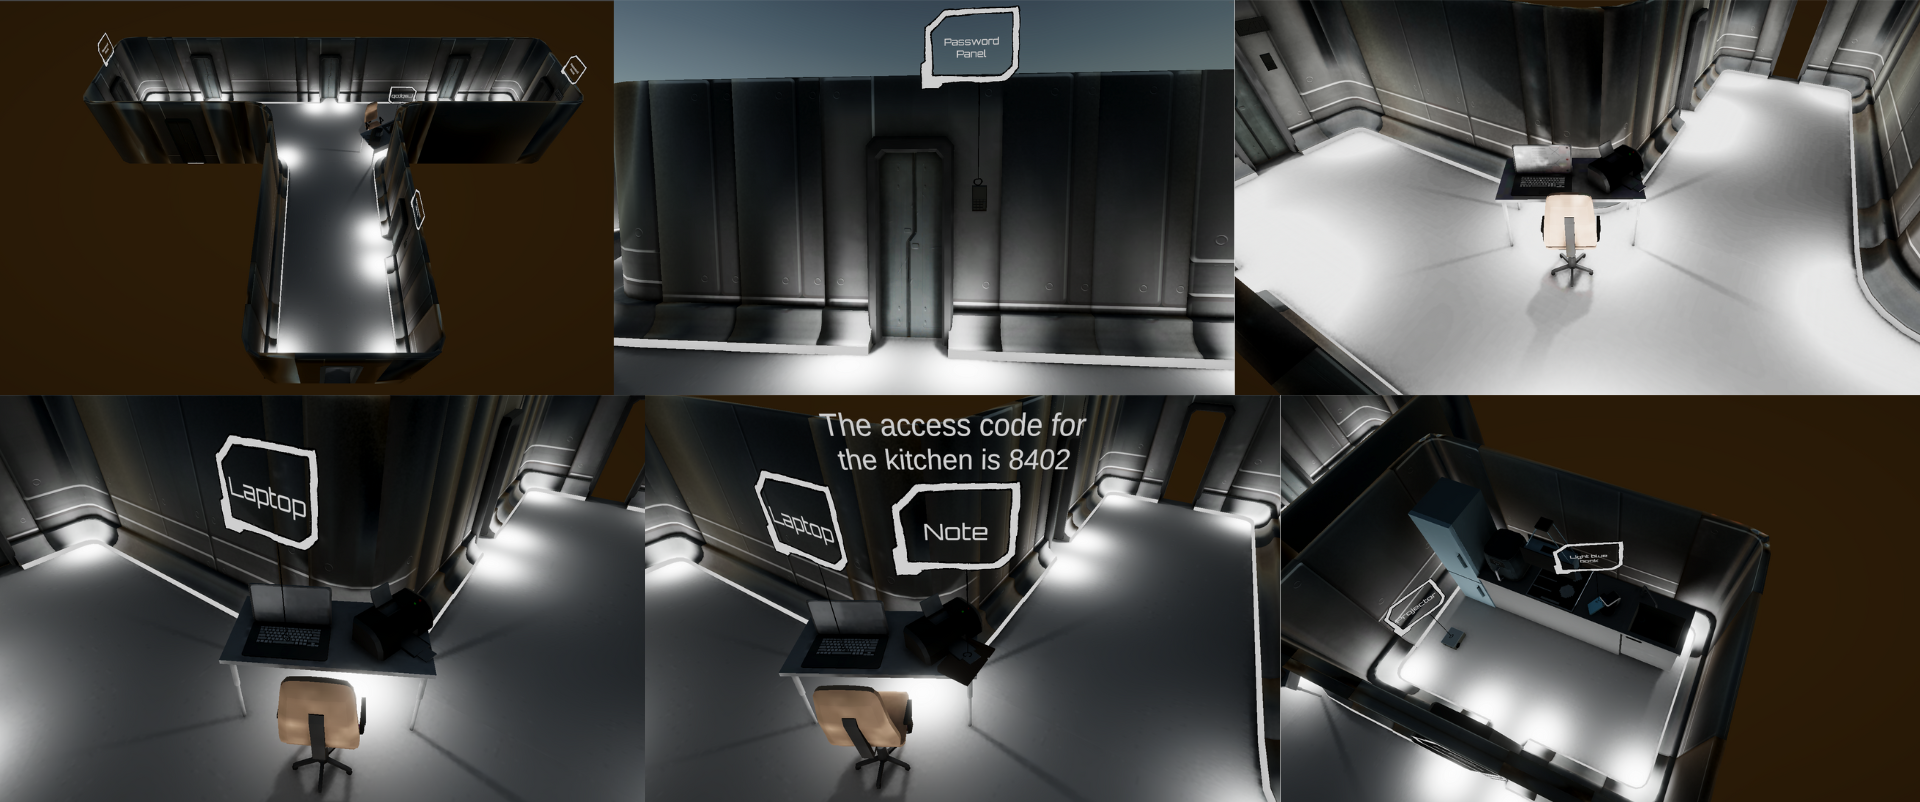
\includegraphics[width=1\linewidth]{content/pictures/Rätseldesign - Abschnitt02 - Rätsel00.png}
\caption{Aufbau der Rätsel von Abschnitt 3, Teil 1 (Quelle: eigene Darstellung)}
\label{fig:riddle-design-section02-00}
\end{figure}

\begin{figure}[ht]
\centering
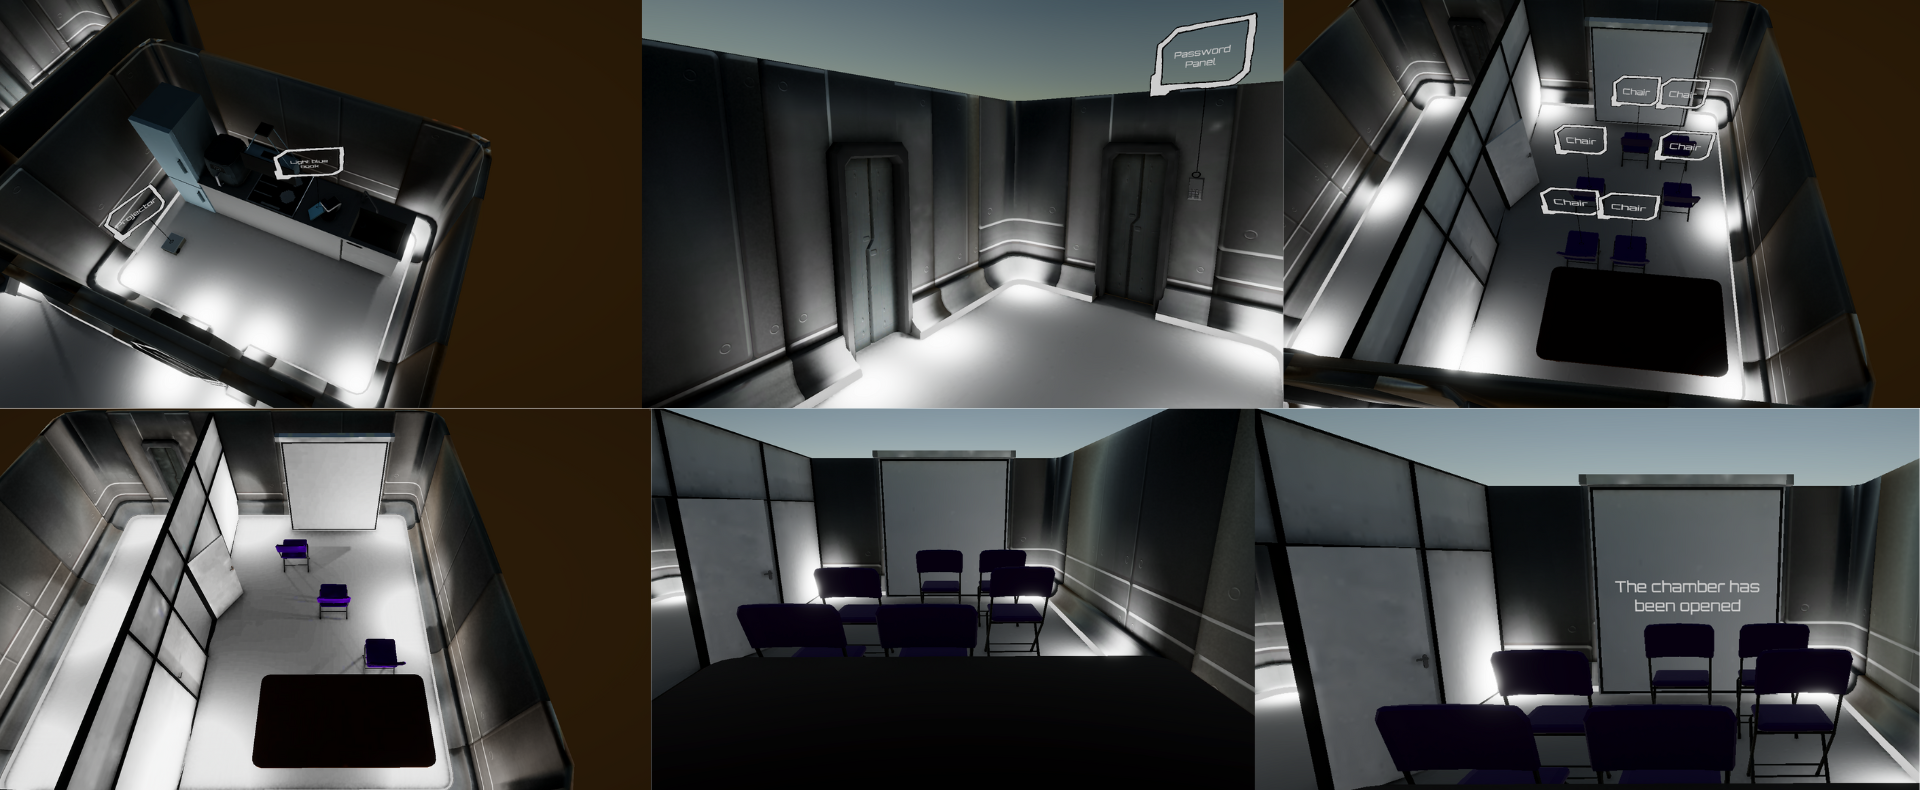
\includegraphics[width=1\linewidth]{content/pictures/Rätseldesign - Abschnitt02 - Rätsel01.png}
\caption{Aufbau der Rätsel von Abschnitt 3, Teil 2 (Quelle: eigene Darstellung)}
\label{fig:riddle-design-section02-0l}
\end{figure}

\begin{figure}[ht]
\centering
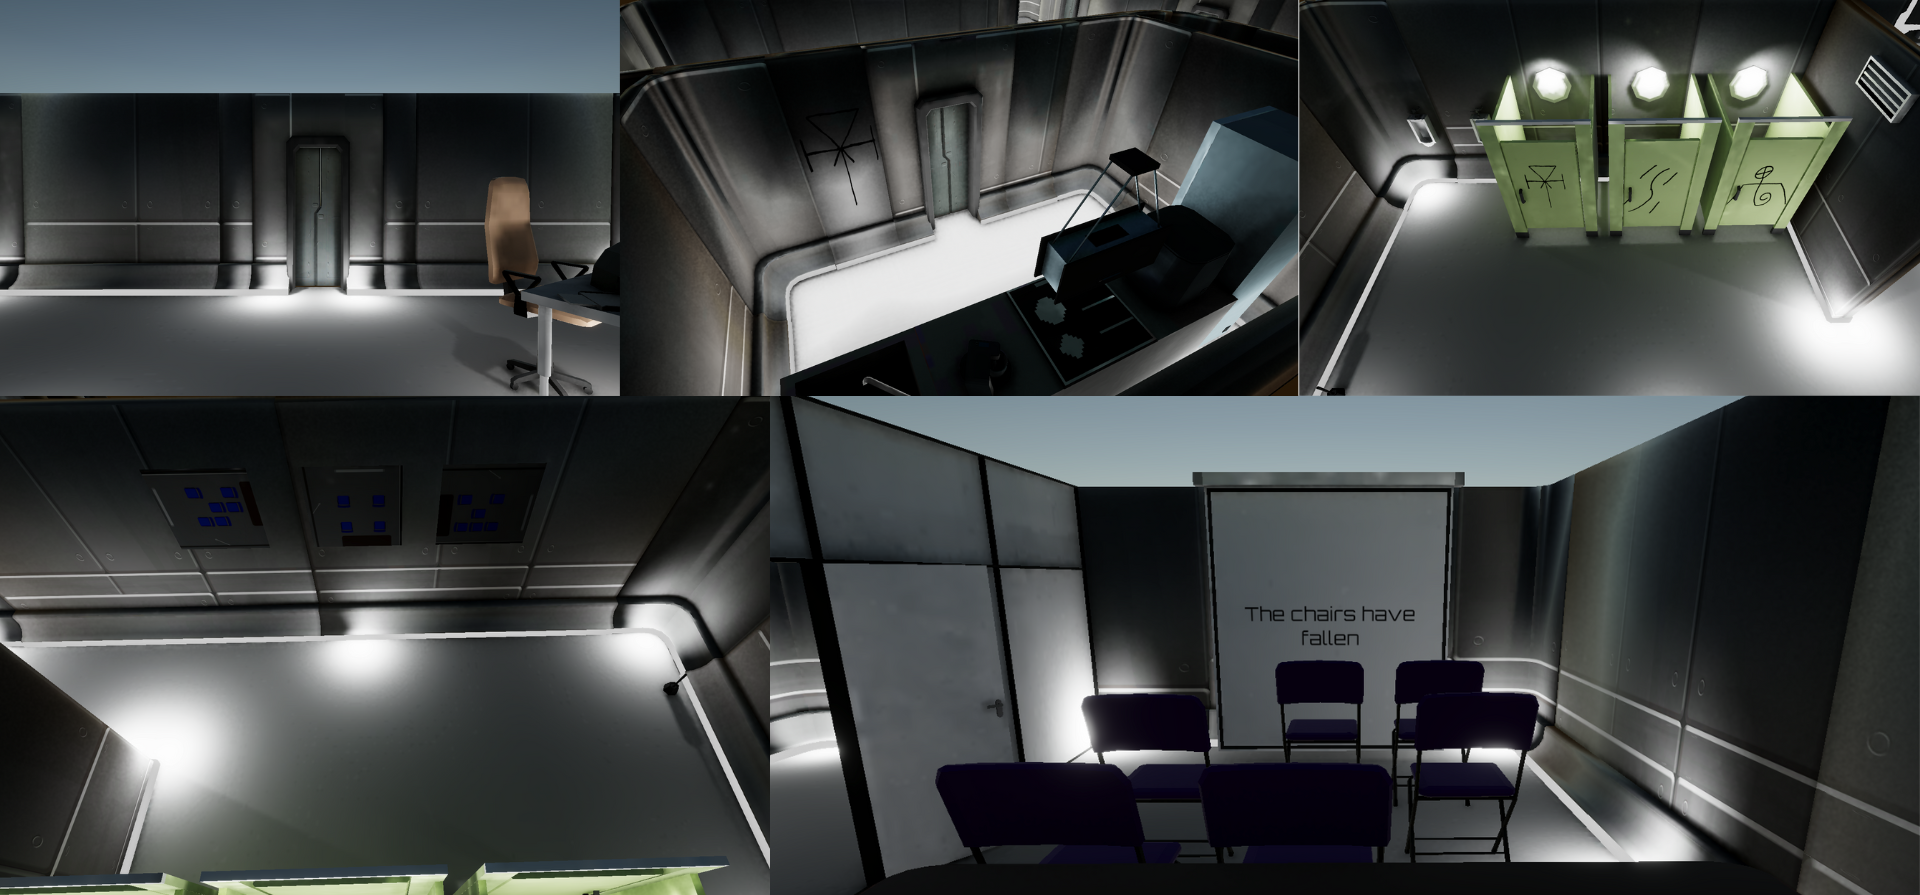
\includegraphics[width=1\linewidth]{content/pictures/Rätseldesign - Abschnitt02 - Rätsel02.png}
\caption{Aufbau der Rätsel von Abschnitt 3, Teil 3 (Quelle: eigene Darstellung)}
\label{fig:riddle-design-section02-02}
\end{figure}

\begin{figure}[ht]
\centering
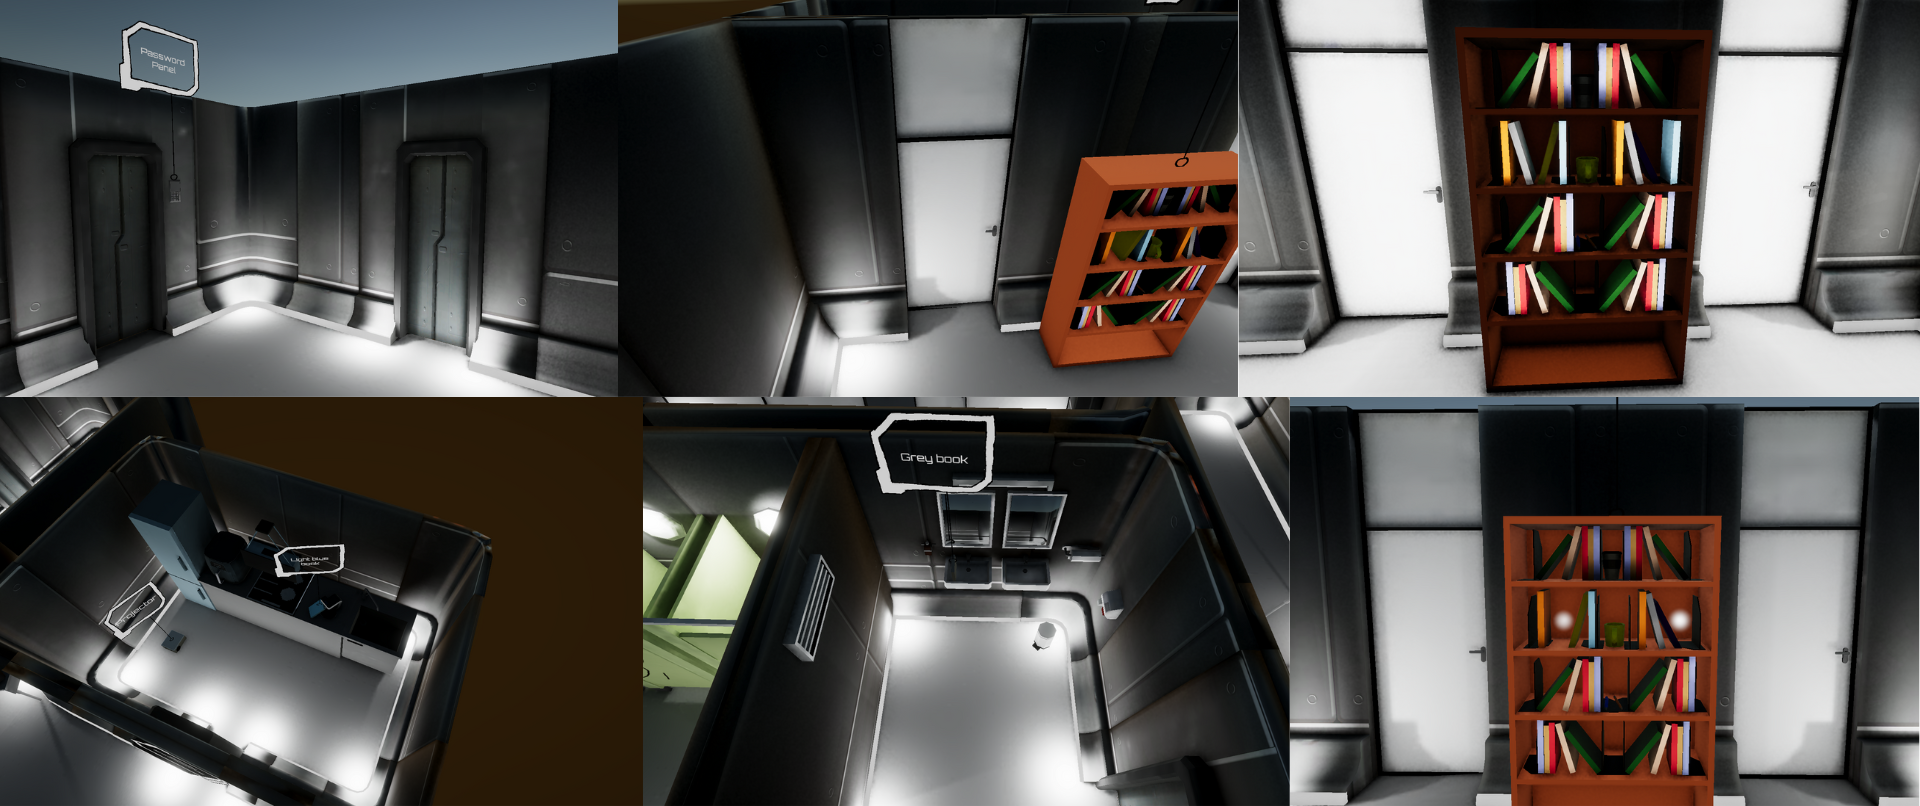
\includegraphics[width=1\linewidth]{content/pictures/Rätseldesign - Abschnitt02 - Rätsel03.png}
\caption{Aufbau der Rätsel von Abschnitt 3, Teil 4 (Quelle: eigene Darstellung)}
\label{fig:riddle-design-section02-03}
\end{figure}

\begin{figure}[ht]
\centering
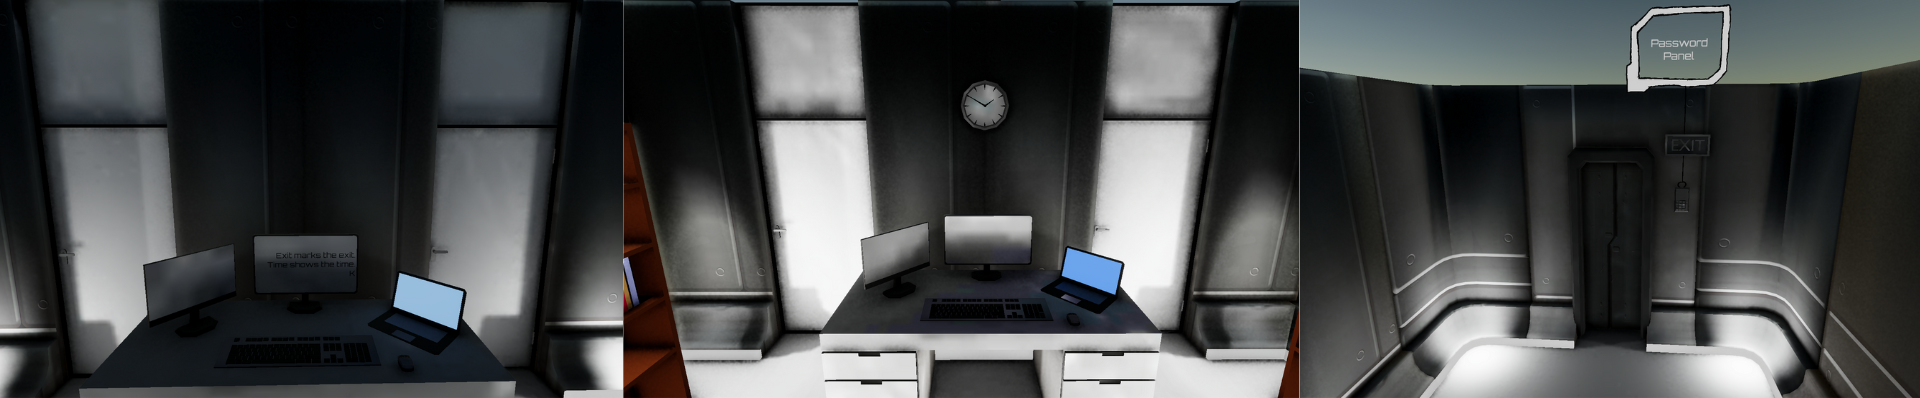
\includegraphics[width=1\linewidth]{content/pictures/Rätseldesign - Abschnitt02 - Rätsel04.png}
\caption{Aufbau der Rätsel von Abschnitt 3, Teil 5 (Quelle: eigene Darstellung)}
\label{fig:riddle-design-section02-04}
\end{figure}

Nachdem der Player den neuen Korridor betreten hat, trifft er auf mehrere verschlossene Türen (vgl. Abbildung \ref{fig:riddle-design-section02-00}, Bild erste Reihe links). Zu Beginn muss der Player den Druckvorgang auslösen, der in der Anwendung des Watchers über einen Laptop im Flur sicht- und ausführbar ist (vgl. Abbildung \ref{fig:riddle-design-section02-00}, Bild zweite Reihe links). Sobald der Druck gestartet wurde, erhält der Player eine Notiz mit einem Zahlencode, der zum Öffnen der Küchentür in der Player-Anwendung benötigt wird (vgl. Abbildung \ref{fig:riddle-design-section02-00}, Bild zweite Reihe Mitte).

Da der Watcher bereits zu diesem Zeitpunkt Zugang zur Küche hat, besteht seine Aufgabe darin, den Player zu dieser zu navigieren. In der Küche findet der Player einen Projektor sowie ein Buch, die in späteren Rätseln von Bedeutung sind (vgl. Abbildung \ref{fig:riddle-design-section02-00}, Bild zweite Reihe rechts). 

Nachdem der Projektor vom Player entdeckt wurde und dieser auch in der Anwendung des Watchers erscheint, wird das Konferenzzimmer zugänglich (vgl. Abbildung \ref{fig:riddle-design-section02-0l}, Bild erste Reihe Mitte und Bild erste Reihe Rechts). Sowohl Player als auch Watcher sehen in diesem Raum mehrere Stühle. Die Anzahl der sichtbaren Stühle unterscheidet sich dabei je nach Anwendung. In der Sicht des Watchers erscheinen zusätzliche Stühle erst dann, wenn der Player sie zuvor entdeckt hat  (vgl. Abbildung \ref{fig:riddle-design-section02-0l}, Bild erste Reihe rechts und zweite Reihe links).

Wird der Projektor vom Watcher auf den Konferenztisch platziert, erscheint eine Nachricht auf der Leinwand. Diese trägt den Text \say{The chamber has been opened}, eine Anspielung auf den Satz aus Harry Potter und die Kammer des Schreckens, und verweist auf das benachbarte Badezimmer, das als nächstes Ziel dient (vgl. Abbildung \ref{fig:riddle-design-section02-0l}, Bild zweite Reihe Mitte und zweite Reihe rechts).

Im Badezimmer erhält der Player einen Hinweis darauf, wie der Watcher die Stühle im Konferenzzimmer anordnen muss. An den Türen der Toilettenkabinen befinden sich drei verschiedene Symbole, die jeweils für eine bestimmte Anordnung der Stühle stehen. Diese Symbole wurden aus dem Spiel We were here too entnommen (vgl. \citealp{total_mayhem_games_we_2018}). Die entsprechenden Anordnungen sind auf Postern dargestellt, die an der Wand des Badezimmers hängen (vgl. Abbildung \ref{fig:riddle-design-section02-02}, Bild erste Reihe rechts und zweite Reihe links).

Welches der drei Symbole für das aktuelle Rätsel relevant ist, kann der Watcher in der Küche erkennen. Es befindet sich auf der Rückwand der Küche zum Flur hin, unmittelbar auf der rechten Seite nach dem Betreten des Raumes (vgl. Abbildung \ref{fig:riddle-design-section02-02}, Bild erste Reihe Mitte). Wenn der Watcher daraufhin die Stühle im Konferenzzimmer entsprechend der richtigen Anordnung platziert, erscheint eine neue Nachricht auf der Leinwand mit dem Text \say{The chairs haven fallen}. Dieser Spruch orientiert sich an dem Lateinischen Ausdruck \say{Alea iacta est}. Diese informiert den Player darüber, dass die Stühle korrekt positioniert wurden und sich nun ein weiterer Raum geöffnet hat (vgl. Abbildung \ref{fig:riddle-design-section02-02}, Bild zweite Reihe rechts).

Am linken Ende des Korridors wird nun ein kleines Büro zugänglich, zu dem sowohl Player als auch Watcher Zutritt erhalten (vgl. Abbildung \ref{fig:riddle-design-section02-03}, Bild erste Reihe links). Dieses Büro existiert in zwei verschiedenen Versionen. Der Player betritt einen Raum auf der einen Seite des Flurs, während sich für den Watcher die Tür auf der gegenüberliegenden Seite öffnet. Obwohl die beiden Büroräume nahezu identisch aufgebaut sind, fehlen dem Player bestimmte Gegenstände, die ergänzt werden müssen.

Beide Büroräume bestehen aus zwei kleinen Unterräumen. Der erste Raum fungiert als kleine Bibliothek, in der sich ein Bücherregal befindet (vgl. Abbildung \ref{fig:riddle-design-section02-03}, Bild erste Reihe Mitte). In der Anwendung des Watchers sind bereits alle Bücher vorhanden, auch jene, die in der Umgebung des Players fehlen (vgl. Abbildungen \ref{fig:riddle-design-section02-03}, Bild zweite Reihe rechts und erste Reihe rechts). Die fehlenden Bücher können in der Küche (vgl. Abbildung \ref{fig:riddle-design-section02-03}, Bild zweite Reihe links), sowie bei den Waschbecken im Badezimmer gefunden werden (vgl. Abbildung \ref{fig:riddle-design-section02-03}, Bild zweite Reihe Mitte).

Werden die Bücher schließlich in der richtigen Reihenfolge in das Regal eingesetzt, das graue Buch links,  das hellblau Buch rechts, öffnet sich die weiße Tür auf der linken Seite, die zum hinteren Bereich des Büros führt (vgl. Abbildung \ref{fig:riddle-design-section02-03}, Bild erste Reihe Mitte).

Der hintere Bereich des Büros bildet den Arbeitsplatz innerhalb des Raums. Dort befinden sich ein Schreibtisch mit einem Computer und mehrere Monitoren. An den seitlichen Wänden sind Bücherregale angebracht, die jedoch für die Lösung des letzten Rätsels keine Relevanz besitzen. Betritt der Player den Raum, kann er auf einem Monitor die Notiz \say{Exit marks the exit. Time shows the time. K.} lesen (vgl. Abbildung \ref{fig:riddle-design-section02-04}, Bild links). Die Notiz enthält einen Hinweis auf das Passwort für den Ausgang und verweist zugleich auf dessen Position innerhalb der Spielwelt.

Zeitgleich wird der hintere Bereich des Büros auch für den Watcher sichtbar. In dieser Version des Raumes ist die Notiz nicht zu sehen; stattdessen befindet sich dort eine Uhr, deren angezeigte Uhrzeit das Passwort für den Ausgang darstellt (vgl. Abbildung \ref{fig:riddle-design-section02-04}, Bild Mitte). Der Ausgang selbst ist durch ein \say{Exit}-Schild gekennzeichnet und befindet sich am rechten Ende des Korridors, unmittelbar neben der Tür zum Konferenzzimmer (vgl. Abbildung \ref{fig:riddle-design-section02-04}, Bild rechts und Abbildung \ref{fig:riddle-design-section02-0l}, Bild erste Reihe Mitte).

Gibt der Player das korrekte Passwort ein, ist das Tutorial abgeschlossen, Infolgedessen können sowohl Player als auch Watcher den entsprechenden Abschnitt des Bürokomplexes verlassen.

\section{Dialoge}

Das grundlegende Spielkonzept sieht einen Dialog vor, der den Spielern Hintergrundinformationen vermittelt und den aktuellen Spielfortschritt erläutert. Im Unterschied zu vielen anderen Spielen ist der Dialog jedoch nicht identisch für beide Spielanwendungen gestaltet. Stattdessen ist vorgesehen, dass die Dialogtexte so aufgeteilt werden, dass sich die Spieler diese gegenseitig vorlesen müssen. Ziel dieses Ansatzes ist es, die wechselseitige Kommunikation zu fördern und die Zusammenarbeit zwischen den Spielteilnehmern gezielt zu stärken.

\section{Sounddesign}

Das Sounddesign soll den visuellen Eindruck der jeweiligen Anwendung durch gezieltes Feedback unterstützen. Sowohl die Bewegung des Playeravatars als auch die Interaktionen des Watchers erzeugen dabei entsprechende akustische Rückmeldungen. Zusätzlich erhalten sowohl Player als auch Watcher über spezifische Klänge ein Feedback, wenn Rätsel erfolgreich gelöst oder neue Wege freigeschaltet wurden.

Die konkrete Ausgestaltung des Sounddesigns wird in den folgenden Unterkategorien näher beschrieben. Grundsätzlich ist das Sounddesign jedoch dezent im Hintergrund gehalten, um die verbale Kommunikation zwischen den Spielern nicht zu beeinträchtigen.

\subsection{Hintergrundmusik}

Jedes Szenario verfügt über eine eigene atmosphärische Hintergrundmusik, die zur akustischen Untermalung der Spielwelt beiträgt. Diese wirkt sich auch auf die klangliche Gestaltung der Geräusche aus, die durch den Avatars des Players sowie durch die Aktionen des Watchers erzeugt werden. So sind beispielsweise Hall-Effekte im leeren Bürokomplex oder ein gedämpfter Klang im Verlies zu hören, die zur jeweiligen räumlichen Atmosphäre beitragen.

Auch das Haupt- und Pausemenü sind mit einer atmosphärischen Klangkulisse unterlegt. Diese dient der Beruhigung und Orientierung, steht jedoch zugleich in thematischem Bezug zum Setting des Spiels.

\subsection{Umgebungsgeräusche}

Jedes dynamische oder licht-emittierende Weltobjekt erzeugt bei Interaktion, Platzierung oder Entfernung ein entsprechendes Geräusch, dessen akustische Eigenschaft, insbesondere der Hall, an die jeweilige Umgehung angepasst sind. Schwere Gegenstände, wie z.B. eine Säule, verursachen beim Abstellen oder Entfernen ein charakteristisches Kratzgeräusch auf dem Boden, das das physikalische Gewicht und die Materialität des Gegenstands auditiv vermittelt.


\subsection{Interaktionsgeräusche}

Jede Interaktion des Players kann mit einem spezifischen Geräusch verknüpft sein. So führt das Tragen einer Fackel in der Kleidung zu einem dezenten Rascheln, wehrend das Einsetzen der Fackel in eine Halterung ein charakteristisches Klacken von Holz auf Metall erzeugt. Auch der Watcher erhält für seine Interaktion innerhalb des Menüs ein auditives Feedback. Sowohl die Auswahl als auch das Verschieben von Gegenständen im Menü werden akustisch begleitet. Bei der Positionsbestimmung eines Gegenstandes ist ein Kratzen oder Schleifen zu hören, das die Bewegung des Gegenstands auditiv nachvollziehbar macht.


\section{Weitere nicht berücksichtigte Überlegungen}

In diesem Kapitel werden Konzeptideen vorgestellt, die im Verlauf der Entwicklung verworfen und nicht in das finale Spielkonzept integriert wurden.

Zu Beginn war vorgesehen, dass in einer Spielsitzung ein Player mit mehreren Watchern gemeinsam interagieren kann. Während der Abschlusspräsentation des vorangegangenen Projekts wurde jedoch hinterfragt, ob sich mehrere Watcher in ihrer Interaktion nicht gegenseitig behindern würden. Als Reaktion auf diese Problematik wurde zunächst erwogen, durch gezielte Events einzelne Watcher temporäre zu beschäftigen, bspw. durch Minispiele, wie sie aus Mobile-Spielen wie \say{Duskwood} oder \say{Sentence} bekannt sind (vgl. \citealp{everbyte_duskwood_2019,jaunt_sentence_2019}). Diese Lösung wurde jedoch verworfen, da sie den Fokus vom eigentlichen Spielkonzept und der Kommunikation der Spieler abgelenkt hätte.

Aus der ursprünglichen Idee ergab sich ein weiteres Konzept, das eine Teamstruktur innerhalb der Spielwelt vorsah. Dabei sollten zwei Gruppen agieren. Ein Team hätte Rätsel in die Spielwelt integriert, während das andere Team sie zu lösen gehabt hätte. Dieses Modell hätte jedoch die Entwicklung einer konsistenten narrativen Struktur erschwert, weshalb auch diese Variante nicht weiterverfolgt wurde.

Im Kontext der angestrebten Gleichwertigkeit zwischen den beiden Spielerrollen wurden weitere Ideen zur Verbesserung der Aufgabenverteilung entwickelt. Eine dieser Überlegungen betraf die Einführung eines Crafting-Systems. Der Player hätte in der Spielwelt verarbeitbare Gegenstände gefunden, die der Watcher in seinem Menü zu leichten oder schweren Gegenständen hätte kombinieren können. Dieser würden zum Lösen und beseitigen der Hindernisse gebraucht werden. Aufgrund des hohen gestalterischen und zeitlichen Aufwands zur Implementierung sowie der begrenzten Relevanz für das zentrale Spielziel wurde diese Idee ebenfalls nicht umgesetzt.

Eine weitere verworfene Idee bezog sich auf ein Notizsystem, das sich an der Kernmechanik des Spiels \say{Shadow of Doubt} orientiert (vgl. \citealp{colepowered_games_shadows_2023}). Der Watcher hätte dabei Notizen, etwa in Form von Screenshots oder Texten, auf einer virtuellen Notiztafel anheften können, basierend auf Beobachtungen oder Informationen, die vom Player gesammelt wurden. Dieses System sollte die Strukturierung der Rätsellogik unterstützen und die Planung der nächsten Spielschritte erleichtern. Auch dieses Feature wurde nicht realisiert, da dem Watcher im späteren Verlauf ohnehin erweiterte Funktionen zur Verfügung stehen (z. B. das Drehen oder Vergrößern von Gegenständen) und das Lösen der Rätsel meist unmittelbar mit dem Platzieren von Gegenständen verknüpft ist. Ein komplexeres Rätseldesign hätte überdies einen erheblichen Mehraufwand in der Entwicklung bedeutet. 